\documentclass[11pt]{article}

\usepackage[T1]{fontenc}
\usepackage{lmodern}
\usepackage[margin=1in]{geometry}
\usepackage{amsmath, amssymb, amsthm}
\usepackage{mathtools}
\usepackage{graphicx}
\usepackage{booktabs}
\usepackage{xurl}
\usepackage{xcolor}
\usepackage{caption}
\usepackage{tabularx}
\usepackage{placeins}
\usepackage{fancyhdr}
\usepackage{natbib}
\usepackage{enumitem}
\usepackage{orcidlink}
\usepackage{tikz}
\usetikzlibrary{arrows.meta, positioning, fit, calc}
\usepackage{hyperref}
\usepackage[capitalise,noabbrev]{cleveref}
\usepackage{thmtools}

\hypersetup{
  colorlinks=true,
  linkcolor=blue!70!black,
  citecolor=green!50!black,
  urlcolor=blue!80!black,
  bookmarksnumbered=true,
  pdfauthor={Ioannis Tsiokos},
  pdftitle={To Plot a Stone with Six Birds: Constructing and Auditing Emergent Geometry from Markov Dynamics}
}

\captionsetup{font=small, labelfont=bf}
\setlist{itemsep=2pt, topsep=4pt}
\setlength{\emergencystretch}{2.5em}

% ---------------------------------------------------------------------------
% Theorem environments
% ---------------------------------------------------------------------------
\declaretheorem[name=Theorem, numberwithin=section, style=plain]{theorem}
\declaretheorem[name=Proposition, sibling=theorem, style=plain]{proposition}
\declaretheorem[name=Lemma, sibling=theorem, style=plain]{lemma}
\declaretheorem[name=Corollary, sibling=theorem, style=plain]{corollary}
\declaretheorem[name=Definition, sibling=theorem, style=definition]{definition}
\declaretheorem[name=Remark, sibling=theorem, style=remark]{remark}

% Provenance line placed after a statement: how the statement is established.
\newcommand{\provenance}[1]{\par\smallskip\noindent{\small\textit{Basis.}~#1}\par\smallskip}
\newcommand{\lean}[1]{\nolinkurl{#1}}

% ---------------------------------------------------------------------------
% Notation
% ---------------------------------------------------------------------------
\newcommand{\R}{\mathbb{R}}
\newcommand{\N}{\mathbb{N}}
\newcommand{\Z}{\mathbb{Z}}
\newcommand{\TV}{\mathrm{TV}}
\newcommand{\RM}{\mathrm{RM}}
\newcommand{\Dist}{\mathrm{Dist}}
\newcommand{\dH}{\dim_{\mathrm{H}}}
\newcommand{\one}{\mathbf{1}}
\newcommand{\Kmac}{K}

\title{To Plot a Stone with Six Birds:\\Constructing and Auditing Emergent Geometry from Markov Dynamics}
\author{Ioannis Tsiokos\,\orcidlink{0009-0009-7659-5964}}
\date{First version (v1): 5 February 2026\\[2pt]
{\small Version 3: 4 October 2026 \quad$\cdot$\quad DOI: \href{https://doi.org/10.5281/zenodo.23130783}{10.5281/zenodo.23130783} \quad$\cdot$\quad v1 DOI: \href{https://doi.org/10.5281/zenodo.18494975}{10.5281/zenodo.18494975}}}

\fancypagestyle{firstpage}{%
  \fancyhf{}
  \fancyfoot[C]{\scriptsize Automorph Inc., Wilmington, DE, USA \quad \texttt{ioannis@automorph.io} \quad DOI: \href{https://doi.org/10.5281/zenodo.23130783}{10.5281/zenodo.23130783} \quad \textcopyright\ 2026 \quad CC-BY 4.0 \quad Preprint --- not peer reviewed.}
  \renewcommand{\headrulewidth}{0pt}
  \renewcommand{\footrulewidth}{0pt}
}

\begin{document}
\maketitle
\thispagestyle{firstpage}

\begin{abstract}
Can points, distances and curvature be built from nothing more than a Markov chain and a decision about what to ignore?
We study this question for finite Markov dynamics within the Six Birds emergence calculus.
A \emph{lens} groups microstates into macro states, each represented by a prototype distribution; lifting, evolving for $\tau$ steps and repackaging gives the macro dynamics.
The distance between two macro states is the cost of the cheapest chain of macro transitions, each step costing the negative logarithm of its symmetrized, floored transition probability.
We prove, and formalize in Lean~4, that this always yields an extended pseudometric, that each macro state's persistence defect equals its escape probability, and that the worst escape probability bounds the closure defect on every microstate.
A layer is \emph{coherent} when its closure, persistence, route and normalized distortion defects all vanish along a declared refinement family.
At stage $\tau=5$ we construct coherent layers, in declared units, for three systems: block lenses on a lazy grid walk, whose normalized metrics converge to the $L^1$ unit square; recursive cells on a Sierpi\'nski gasket walk, converging to a self-similar compact space of Hausdorff dimension $\log 3/\log 2$ in which arbitrarily small balls about every point resist Hilbert approximation to within one sixteenth of their radius; and reservoir chains on the sphere, converging to the round unit sphere, whose curvature a landmark transport estimator recovers from the Markov metrics.
For the isotropic walk on the lattice, centred negative-log probabilities converge uniformly to a quadratic form on diffusive windows, so the square root of the cost, in diffusive units, converges to Euclidean distance and the Pythagorean identity becomes a law of accounting.
The analysis also marks the limits of the approach.
Spectrally learned lenses give valid metrics but fail persistence, for the canonical grid and gasket partitions under every choice of prototype, and a local-MDS holonomy estimator can overestimate curvature by more than $20\%$ in the refinement limit, even on exact spherical distances.
\end{abstract}

\noindent\textbf{Keywords:} emergent geometry; Markov chains; coarse-graining; likelihood path metrics; holonomy; Sierpi\'nski gasket; local limit theorem; Lean~4; emergence calculus

\section{Introduction}
\label{sec:introduction}

To \emph{plot} a stone is to treat it as if it already lives in a space: we give it a location, measure how far it is from other things, and speak of the surface it rests on as flat or curved.
Yet nobody observes space directly.
What an observer has is narrower: a record of how configurations change, and an interface that can tell some configurations apart and not others.
Six Birds Theory (SBT)~\cite{SixBirdsTheory} takes this seriously and treats points, distances and geometric laws not as primitives but as \emph{closure artifacts}: structures that become available when repeated compression of a dynamics stabilizes.
This paper asks what that means concretely.
Starting from a finite Markov chain and nothing else, when can one construct points, a distance, and a notion of curvature, and how can one tell whether the result deserves to be called a geometry?

\paragraph{The construction in one paragraph.}
Microstates are grouped into blocks by a \emph{lens}; the blocks are the candidate points.
Each block is represented by a \emph{prototype}, a probability distribution on its microstates.
Lifting a block to its prototype, running the micro dynamics for $\tau$ steps, and recording which block the walker lands in gives a Markov kernel between blocks.
Transition probabilities are symmetrized, each macro transition is assigned a cost, the negative logarithm of its symmetrized probability (floored away from zero), and the distance between two blocks is the cost of the cheapest chain of transitions connecting them.
\Cref{fig:pipeline} summarizes the pipeline.
Nothing in it refers to coordinates: whatever geometry appears is produced by the dynamics, the choice of lens, and the accounting rule.

\begin{figure}[t]
\centering
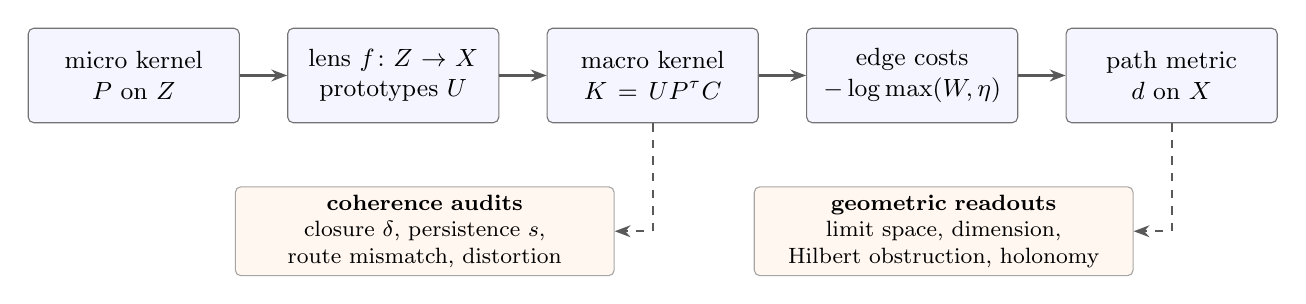
\begin{tikzpicture}[
  node distance=5mm and 6mm,
  stage/.style={draw=black!55, rounded corners=2pt, fill=blue!4, align=center, font=\small, inner sep=4pt, minimum height=12mm, text width=24mm},
  audit/.style={draw=black!35, rounded corners=2pt, fill=orange!6, align=center, font=\footnotesize, inner sep=3pt, text width=46mm},
  arr/.style={-{Stealth[length=2mm]}, black!65, thick}
]
\node[stage] (micro) {micro kernel\\$P$ on $Z$};
\node[stage, right=of micro] (lens) {lens $f\colon Z\to X$\\prototypes $U$};
\node[stage, right=of lens] (macro) {macro kernel\\$K=UP^{\tau}C$};
\node[stage, right=of macro] (cost) {edge costs\\$-\log\max(W,\eta)$};
\node[stage, right=of cost] (metric) {path metric\\$d$ on $X$};
\draw[arr] (micro) -- (lens);
\draw[arr] (lens) -- (macro);
\draw[arr] (macro) -- (cost);
\draw[arr] (cost) -- (metric);
\node[audit, below=8mm of lens, xshift=4mm] (gates) {\textbf{coherence audits}\\closure $\delta$, persistence $s$,\\route mismatch, distortion};
\node[audit, below=8mm of cost, xshift=4mm] (readouts) {\textbf{geometric readouts}\\limit space, dimension,\\Hilbert obstruction, holonomy};
\draw[arr, dashed] (macro.south) |- (gates.east);
\draw[arr, dashed] (metric.south) |- (readouts.east);
\end{tikzpicture}
\caption{From dynamics to a metric. A lens groups microstates into macro states, prototypes lift macro states back to distributions, and staging for $\tau$ steps gives the macro kernel $K$. Symmetrized macro transition probabilities $W$ are converted into nonnegative edge costs, and the distance is the cheapest protocol (path) cost. Audits test whether the layer closes and persists; readouts describe the geometry it produces.}
\label{fig:pipeline}
\end{figure}

\paragraph{When is it a geometry?}
Any lens produces a distance matrix, so a distance matrix alone proves nothing.
We require \emph{coherence}: the packaged layer must close (repackaging does not drift), its points must persist (prototypes are nearly fixed by the closed dynamics), and the induced distances must agree across a family of refining lenses once units are declared.
\Cref{sec:closure} makes this precise.
A central lesson of the paper is that coherence must be stated as a limit along an explicit refinement family, with explicit distance units: finite defect values, and phrases such as ``bounded defect'', carry no information on their own, because every total-variation defect is at most one and every distortion on a connected finite graph is finite.

\paragraph{What the paper establishes.}
\begin{enumerate}[leftmargin=*]
\item \textbf{Foundations} (\cref{sec:construction,sec:closure}).
The likelihood path distance is always an extended pseudometric, and identifying points at distance zero gives an extended metric.
The closure and macro kernels are stochastic; a prototype's persistence defect equals its macro escape probability; and the worst escape is an upper bound on the closure defect on every microstate.
These statements are mechanized in Lean~4.
\item \textbf{Three coherent regimes} (\cref{sec:constructed}).
With the original stage $\tau=5$, we construct nested lenses whose closure, persistence, route and normalized distortion defects vanish together, and identify the limit of the normalized metrics: block lenses on the original lazy grid walk (limit: the $L^1$ unit square); recursive cells on the original lazy gasket walk (limit: a compact self-similar space of Hausdorff dimension $\log 3/\log 2$, in which every ball of radius $2^{-j}$ about every point admits no Hilbert approximation with distance error at most $2^{-j}/16$); and nested cube cells on a new family of spherical reservoir chains (limit: the round unit sphere).
\item \textbf{Curvature as route dependence of transport} (\cref{sec:curvature}).
Holonomy is identified exactly with the noncommutation of covariant transport operators on a common section space, and a supplied spherical connection obeys an exact area law.
The local-MDS and Procrustes holonomy estimator used in our pipeline is gauge invariant and separates our flat and curved test substrates, but it is not a consistent curvature estimator: on exact spherical distances its area-normalized output can converge to $\approx1.2032$ or to $0$ instead of $1$.
A landmark-based transport estimator does converge, and the reservoir construction supplies the metric-error rate needed to apply it to actual Markov metrics.
\item \textbf{Pythagoras as accounting} (\cref{sec:pythagoras}).
For the isotropic lazy walk on the lattice $\Z^2$, a Fourier local limit estimate shows that the centred negative-log probability $F_n(z)$ after $n$ steps satisfies $|F_n(z)-2|z|^2/n|\to0$ uniformly on central windows $|z|\le R\sqrt n$, with explicit error bounds.
Hence the readout $\sqrt{F_n(z)/2}$ converges uniformly to the Euclidean length $|z|/\sqrt n$ in diffusive units, and the coordinate-axis Pythagorean residual vanishes.
A matched walk with correlated steps keeps a quadratic cost, but at the diagonal displacement $x=y=\lfloor\sqrt n\rfloor$ its axis residual tends to $-16/5$.
\item \textbf{An audit of learned lenses} (\cref{sec:learned}).
Lens ladders learned by spectral clustering give valid finite metrics with measurable, constraint-sensitive structure, but their finest levels have worst prototype defects of about $0.78$ (grid), $0.99$ (sphere) and $0.85$ (gasket).
For the grid and gasket partitions no choice of prototypes can lower the worst defect.
\end{enumerate}

\begin{table}[t]
\centering
\small
\caption{Summary of the regimes studied. ``Original'' dynamics are the lazy walks used throughout the paper; all lens families use stage $\tau=5$. Coherence means that closure, persistence, route and normalized distortion defects tend to zero together along the stated family (\cref{def:coherence}).}
\label{tab:summary}
\begin{tabularx}{\textwidth}{@{}>{\raggedright\arraybackslash}p{0.17\textwidth}>{\raggedright\arraybackslash}p{0.17\textwidth}>{\raggedright\arraybackslash}p{0.14\textwidth}>{\raggedright\arraybackslash}X>{\raggedright\arraybackslash}p{0.12\textwidth}@{}}
\toprule
Regime & Micro dynamics & Lens & Outcome & Section \\
\midrule
Grid & original open-grid walk & nested blocks (supplied) & coherent; normalized metrics converge to the $L^1$ unit square & \cref{sec:grid} \\
Gasket & original gasket walk & recursive cells (supplied) & coherent; normalized metrics converge to a compact self-similar space, $\dH=\log 3/\log 2$, with a quantitative local Hilbert obstruction & \cref{sec:gasket} \\
Sphere & spherical reservoir chains (new) & nested cube cells (supplied) & coherent, including routes from every microstate; normalized metrics converge to the unit sphere; transport recovers curvature $1$ & \cref{sec:sphere,sec:transport-repair} \\
Learned ladders & original grid, gasket, gated grid; sphere $k$NN walk & spectral $k$-means & valid finite metrics; persistence fails at fine levels & \cref{sec:learned} \\
Staged accounting & original isotropic walk on $\Z^2$ & none (displacement) & centred cost $\to2|z|^2/n$ on diffusive windows; square-root readout $\to$ Euclidean distance & \cref{sec:pythagoras} \\
\bottomrule
\end{tabularx}
\end{table}

\Cref{tab:summary} collects these outcomes.
Two features deserve emphasis.
First, the coherent lenses are \emph{supplied}: they are written down using the structure of each substrate, not discovered from the kernel.
The constructions therefore establish that coherent geometric layers exist under the stated dynamics, not that they can be found automatically.
Second, the same local rule (hold with probability $\tfrac12$, otherwise step to a uniformly chosen neighbour) yields two different geometries depending on the readout.
Under block lenses on the open grid, where only the boundary convention differs, the normalized protocol (shortest-path) metric converges to $L^1$ distance, whereas on the lattice the one-shot likelihood of a long staged displacement is asymptotically quadratic, and its square-root readout yields Euclidean distance.
Which geometry ``emerges'' depends on how moves are composed and costed, a point we return to in \cref{sec:conclusion}.

\paragraph{How the claims are established.}
The paper uses four kinds of evidence, and each result states which ones it rests on in a short line beginning \emph{Basis}.
\emph{Lean} means the statement, or the named bridge within its proof, is mechanized in Lean~4 against mathlib, with only the standard axioms (\cref{app:lean}).
\emph{Written proof} means a conventional mathematical proof, given in the text or in \cref{app:proofs}.
\emph{Exact computation} means a finite certificate checked in integer or rational arithmetic by a verifier that rebuilds it from the stated inputs.
\emph{Floating computation} means an ordinary numerical experiment.
Finite computations illustrate and check the universal arguments; they never substitute for them.

\paragraph{Relation to other work.}
This paper is the geometric instantiation of the emergence calculus of~\cite{SixBirdsTheory} and a companion to our treatment of emergent counting~\cite{ToCountAStone}.
It draws on standard tools: Markov chains~\cite{Norris1997}, diffusion maps and spectral clustering for learned lenses~\cite{CoifmanLafon2006,vonLuxburg2007,Lloyd1982}, classical multidimensional scaling and Procrustes alignment~\cite{BorgGroenen2005,Schonemann1966}, Riemannian holonomy~\cite{Lee1997Riemannian}, fractal geometry~\cite{Falconer2003Fractal}, metric convergence~\cite{Gromov1999Metric}, and local limit theorems~\cite{Durrett2019Probability}.

\paragraph{Roadmap.}
\Cref{sec:six-birds} recalls the six primitives and how they specialize to geometry.
\Cref{sec:construction} defines the construction and proves its metric properties.
\Cref{sec:closure} develops closure theory and states the coherence criterion.
\Cref{sec:learned} audits learned spectral ladders, and \cref{sec:constructed} constructs the three coherent regimes.
\Cref{sec:curvature} treats curvature, \cref{sec:pythagoras} the Pythagorean law, and \cref{sec:limits} robustness and scope.
\Cref{sec:conclusion} interprets the results.
The appendices contain the Lean map, proof details, reproduction instructions and the version history.
All code, configurations, certificates and audit records are available at \url{https://github.com/ioannist/six-birds-space}.

\section{Six Birds: how the primitives specialize to geometry}
\label{sec:six-birds}

Six Birds Theory~\cite{SixBirdsTheory} describes how a higher layer of description (a ``theory'' in its technical sense: a lens, a completion and an audit) becomes available when repeated compression of a lower layer stabilizes.
It identifies six primitives.
The primitives are unchanged here; what changes is the object they produce.
For counting, the stable object is quantity~\cite{ToCountAStone}; for plotting, it is location, distance and transport.
This section states the correspondence informally; later sections make each item precise.

\paragraph{P1, operator rewrite (closure).}
A layer is usable only if its dynamics can be written in its own variables without reopening micro detail.
Here this is the macro kernel $K=UP^{\tau}C$ and the closure operator $E=P^{\tau}CU$ on micro distributions.
Closure is not assumed; its defect is measured (\cref{sec:closure}).

\paragraph{P2, constraints (feasibility).}
Constraints decide which transitions are possible and how likely they are.
Geometrically they shape neighbourhoods and anisotropy.
Gating moves in one direction deforms the induced metric even when the lens is held fixed (\cref{sec:anisotropy}).

\paragraph{P3, protocols (order of composition).}
A protocol is a chain of moves.
Distance is the cheapest protocol between two points, and curvature is the dependence of transport on the route taken: carrying a frame around a loop need not return it unchanged.
\Cref{sec:curvature} shows that this route dependence is exactly the failure of two covariant transport operators to commute, a statement that remains meaningful even though planar rotations themselves commute.

\paragraph{P4, staging (multi-scale refinement).}
Staging supplies the time parameter $\tau$ and a ladder of refining lenses.
Geometry is claimed only for structure that persists along a declared refinement family; in our constructions both the substrate and the lens are refined jointly.

\paragraph{P5, packaging (quotienting indistinguishability).}
Packaging maps many microstates to one macro state.
This is where points come from: a point is a block of microstates that the interface does not distinguish at the chosen resolution.

\paragraph{P6, accounting (cost).}
Accounting assigns a cost to each move.
Our cost is the negative log-probability of a macro transition, so distance is a ledger rather than a ruler.
Different ways of composing the same ledger give different geometries: chained macro transitions give an $L^1$ metric on the grid, while the one-shot cost of a long staged displacement is quadratic and gives Euclidean distance (\cref{sec:pythagoras}).

\begin{table}[t]
\centering
\small
\caption{The six primitives and their role in this paper.}
\label{tab:six-birds-geometry}
\begin{tabularx}{\textwidth}{@{}>{\raggedright\arraybackslash}p{0.2\textwidth}X@{}}
\toprule
Primitive & Role in emergent geometry \\
\midrule
P1 Operator rewrite & Macro kernel and closure operator; closure and persistence defects (\cref{sec:closure}). \\
P2 Constraints & Feasible moves; anisotropy and deformation of the induced metric (\cref{sec:anisotropy}). \\
P3 Protocols & Distance as cheapest protocol; curvature as route dependence of transport (\cref{sec:construction,sec:curvature}). \\
P4 Staging & Stage $\tau$ and refinement families; coherence as a joint limit (\cref{sec:closure,sec:constructed}). \\
P5 Packaging & Points as blocks of microstates; supplied versus learned lenses (\cref{sec:learned,sec:constructed}). \\
P6 Accounting & Negative-log costs; quadratic accounting and the Pythagorean law (\cref{sec:construction,sec:pythagoras}). \\
\bottomrule
\end{tabularx}
\end{table}

\section{The construction: from packaging to a metric}
\label{sec:construction}

This section defines the objects used throughout and proves the basic metric facts.
Nothing here depends on a particular substrate.

\subsection{Micro dynamics, lenses and prototypes}

Let $Z$ be a finite nonempty set of microstates and $P\in\R^{Z\times Z}$ a row-stochastic Markov kernel~\cite{Norris1997}.
Distributions are row vectors, so one step maps $\mu$ to $\mu P$, and the stage parameter $\tau\in\N$ gives the $\tau$-step map $\mu\mapsto\mu P^{\tau}$.

A \emph{lens} is a map $f\colon Z\to X$ onto a finite set $X$ of macro states (nonempty, since $f$ is onto).
Its fibres $f^{-1}(x)$ are the blocks of microstates that the lens does not distinguish; they are the candidate \emph{points} at this resolution.
The lens is encoded by the deterministic coarse matrix $C\in\{0,1\}^{Z\times X}$, $C[z,x]=\one\{f(z)=x\}$, which pushes a micro distribution $\mu$ forward to $\mu C$.

To go back from macro to micro we choose, for each $x\in X$, a \emph{prototype} $u_x$, a probability distribution on $Z$.
The prototypes form the rows of a stochastic matrix $U\in\R^{X\times Z}$.
We always use prototypes supported on their own fibres, $u_x(z)=0$ whenever $f(z)\neq x$.
Then every fibre is nonempty and
\begin{equation}
UC=I_X,
\label{eq:UC}
\end{equation}
so lifting a macro distribution and repackaging it returns the same macro distribution.
Two prototype choices are used: \emph{uniform} on the fibre, and \emph{stationary-conditional}, which restricts a chosen stationary law $\pi$ of $P$ to the fibre and renormalizes; the latter requires $\pi(f^{-1}(x))>0$ for every $x$.

\subsection{Closure and the macro kernel}

Lifting, evolving for $\tau$ steps and repackaging defines two operators:
\begin{equation}
E \coloneqq P^{\tau}CU \in\R^{Z\times Z},
\qquad
K \coloneqq UP^{\tau}C \in\R^{X\times X}.
\label{eq:closure-macro}
\end{equation}
$E$ is the \emph{closure} acting on micro distributions (evolve, repackage, re-lift), and $K$ is the \emph{macro kernel}: $K_{xy}$ is the probability that a walker started from prototype $u_x$ is in block $y$ after $\tau$ steps.
Both are row-stochastic whenever $P$ and $U$ are (\cref{prop:closure-basic}).
This is the simplest form of the operator-rewrite primitive: micro dynamics rewritten in macro variables by inserting a packaging map and a chosen lift.

\subsection{Likelihood costs}
\label{sec:costs}

To obtain an undirected geometry we symmetrize macro transition probabilities into a weight array
\begin{equation}
W\coloneqq \tfrac12\bigl(K+K^{\mathsf T}\bigr),
\end{equation}
which is symmetric with entries in $[0,1]$ (it need not be stochastic).
Fix a probability floor $0<\eta\le 1$ and an edge threshold $\varepsilon_{\mathrm{edge}}\ge 0$.
For $x\neq y$ the edge $\{x,y\}$ is present when $W_{xy}>\varepsilon_{\mathrm{edge}}$, and then its cost is
\begin{equation}
c(x,y)\coloneqq -\log\max\bigl(W_{xy},\eta\bigr)\ \in\ [0,\,-\log\eta].
\label{eq:cost}
\end{equation}
Absent edges have cost $+\infty$.
The floor only caps the cost of very unlikely present edges; it never creates an edge.
Costs are nonnegative because $\max(W_{xy},\eta)\le 1$.

\begin{remark}[Why a floor and not additive smoothing]
The superficially similar rule $-\log(W_{xy}+\eta)$ is negative whenever $W_{xy}+\eta>1$, for instance when $W_{xy}=1$.
A negative undirected edge creates negative-cost cycles, so the infimum over paths can be $-\infty$ and shortest-path algorithms are invalid.
The floor rule~\eqref{eq:cost} avoids this.
In the limit constructions of \cref{sec:constructed} the floor is chosen below every positive edge weight, so it is inactive; a fixed positive floor would eventually clip edges of a refining family whose transition probabilities tend to zero.
\end{remark}

\subsection{Distance as cheapest protocol}

A \emph{protocol} from $x$ to $y$ is a finite path $\gamma=(x=x_0,x_1,\dots,x_k=y)$ in the macro graph, including the empty path when $x=y$.
Its cost is additive, $\mathrm{Cost}(\gamma)=\sum_{i<k}c(x_i,x_{i+1})$, and the induced distance is
\begin{equation}
d(x,y)\coloneqq \inf_{\gamma\colon x\rightsquigarrow y}\mathrm{Cost}(\gamma)\ \in[0,\infty].
\label{eq:path-metric}
\end{equation}
In computation, $d$ is obtained by an all-pairs shortest-path search.
Edges of cost exactly zero must be kept as edges: treating them as absent would disconnect precisely the zero-distance classes that \cref{prop:metric} identifies.

\begin{proposition}[The likelihood path distance]
\label{prop:metric}
For every finite macro kernel $K$, floor $0<\eta\le1$ and threshold $\varepsilon_{\mathrm{edge}}\ge0$:
\begin{enumerate}[label=(\roman*)]
\item $d$ is an extended pseudometric on $X$: $d(x,x)=0$, $d(x,y)=d(y,x)$, and $d(x,z)\le d(x,y)+d(y,z)$, with values in $[0,\infty]$.
\item $d(x,y)<\infty$ for all $x,y$ if and only if the macro graph is connected.
\item Identifying points at distance zero gives an extended metric space whose distances are those of $d$.
It is an ordinary metric space exactly when the graph is connected.
\end{enumerate}
\end{proposition}

\begin{proof}
The empty protocol gives $d(x,x)=0$.
Concatenating a protocol from $x$ to $y$ with one from $y$ to $z$ gives a protocol from $x$ to $z$ whose cost is the sum, which yields the triangle inequality after taking infima; reversing a protocol preserves its cost because $c$ is symmetric.
Nonnegativity of~\eqref{eq:cost} keeps all values in $[0,\infty]$.
Part (ii) is immediate from the definition, since only absent edges have infinite cost.
Part (iii) is the separation quotient of an extended pseudometric.
\end{proof}

\provenance{Lean: weighted protocols and their costs are defined in \lean{PathMetric.lean}, which proves \lean{weightedEdist_self}, \lean{weightedEdist_triangle}, \lean{weightedEdist_symm} and builds \lean{weightedPseudoEMetricSpace} without assuming connectivity, positive costs or separation. \lean{weightedSeparationMetric} applies the separation quotient of \lean{QuotientMetric.lean} to this distance, and \lean{flooredLikelihoodCost_nonneg} proves nonnegativity of~\eqref{eq:cost} for $W\le1$ and $0<\eta\le1$.}

Zero distances between distinct points do occur.
For the two-state deterministic swap with threshold $\varepsilon_{\mathrm{edge}}<1$ (for instance $0$), both off-diagonal probabilities equal one, so both edges are present with cost zero and the two states are at distance zero.
Separation is therefore a property to be checked, not assumed.
The constructions of \cref{sec:constructed} prove explicit positive lower bounds on all edge costs together with connectivity, which gives separation and finiteness directly.

\begin{remark}[Directed costs]
Using $K$ instead of $W$ gives a directed shortest-path distance, an extended quasi-pseudometric: it satisfies the triangle inequality but need not be symmetric, and distinct points may again be at distance zero.
Directed geometries are natural under asymmetric constraints but are not studied here.
\end{remark}

\section{Closure, persistence and coherence}
\label{sec:closure}

A lens always produces a distance matrix.
This section introduces the audits that decide whether the packaged layer behaves like a stable description, proves the identities that make them computable, and states the coherence criterion used in the rest of the paper.
Throughout, $\TV(\mu,\nu)=\tfrac12\|\mu-\nu\|_1$ is total variation distance.

\subsection{Closure and persistence defects}

The closure $E$ of~\eqref{eq:closure-macro} would be a projection if applying it twice changed nothing.
We measure the departure from idempotence by the worst case over point masses,
\begin{equation}
\delta\coloneqq \max_{z\in Z}\TV\bigl(\delta_zE^2,\ \delta_zE\bigr).
\label{eq:delta}
\end{equation}
Every distribution is a convex combination of point masses, so the same number bounds $\TV(\mu E^2,\mu E)$ for every distribution $\mu$, and the bound is attained.
Points should also persist: the closed dynamics should nearly fix each prototype.
The \emph{prototype} (persistence) \emph{defect} of $x\in X$ is
\begin{equation}
s(x)\coloneqq \TV\bigl(u_xE,\ u_x\bigr),
\label{eq:stability}
\end{equation}
and we report its mean and its worst case $\max_x s(x)$.
The \emph{escape probability} of $x$ is $1-K_{xx}$, the probability that a walker started from $u_x$ is outside block $x$ after $\tau$ steps.

\begin{proposition}[Closure identities]
\label{prop:closure-basic}
Let $P$ and $U$ be stochastic and let the prototypes be supported on their fibres.
\begin{enumerate}[label=(\roman*)]
\item $E$ and $K$ are stochastic, and $UC=I$.
\item Lifting by $U$ preserves the $\ell^1$ norm of every signed macro vector: $\|vU\|_1=\|v\|_1$.
\item Each prototype defect equals the escape probability: $s(x)=1-K_{xx}$.
\item The closure defect on every microstate is bounded by the worst escape:
$\delta\le\max_{x}(1-K_{xx})$.
\item For every distribution $\mu$ and $k\in\N$, $\TV(\mu E^{k+1},\mu E)\le k\,\delta$.
\end{enumerate}
\end{proposition}

\begin{proof}
(i) Products of stochastic matrices are stochastic, $C$ is stochastic because $f$ is a function, and fibre support gives $UC=I$.
(ii) The rows of $U$ have disjoint supports and unit mass, so $\|vU\|_1=\sum_x|v_x|\,\|u_x\|_1=\|v\|_1$.
(iii) Write $B=P^{\tau}C$, so $E=BU$ and $K=UB$.
Then $u_xE-u_x=(K_{x\cdot}-e_x)U$, and by (ii) its total variation is $\tfrac12\|K_{x\cdot}-e_x\|_1=1-K_{xx}$.
(iv) The identity $E^2-E=(BU)^2-BU=(B(UB)-B)U=B(K-I)U$ shows that row $z$ of $E^2-E$ is $(B_{z\cdot}(K-I))U$.
By (ii) its total variation is $\tfrac12\|B_{z\cdot}(K-I)\|_1$; as $B_{z\cdot}$ is a distribution, convexity bounds this by $\max_x\tfrac12\|K_{x\cdot}-e_x\|_1=\max_x(1-K_{xx})$.
(v) By induction, using $\TV(\mu E^{j+1},\mu E^{j})\le\delta$ for the distribution $\mu E^{j-1}$ and the triangle inequality.
\end{proof}

\provenance{Lean: \lean{closure_and_macro_stochastic}, \lean{lift_coarse_identity}, \lean{fiber_push_l1_isometry}, \lean{prototype_stability_eq_escape}, \lean{closure_defect_factorization}, \lean{closure_defect_le_macro_escape}, \lean{totalVariation_extreme_point_iff} and \lean{closure_repetition_bound} in \lean{MarkovClosure.lean}.}

Part (iv) is the workhorse of \cref{sec:constructed}: to control closure on \emph{every} microstate it suffices to bound how much probability leaves each block, which is a statement about the prototypes alone.
Part (v) is deliberately weak.
Repeating the closure $k$ times can drift by up to $k\delta$ (and trivially by at most $1$); nothing in this paper provides a bound that is both small and uniform in the number of repetitions.

Two cautions shape the coherence criterion below.
First, every total-variation defect lies in $[0,1]$, so saying that $\delta$ is ``bounded'' says nothing; only smallness relative to a declared tolerance, or convergence to zero along a family, is informative.
Second, persistence cannot be demanded all the way down to single microstates.
For the lazy grid walk (holding probability $\tfrac12$) on a grid of side at least two, with singleton fibres ($C=U=I$, $\tau=1$), every prototype defect is $1-P_{zz}=\tfrac12$, whatever the grid size.
Conversely, a small idempotence defect does not imply persistence: the two-state kernel with all entries $\tfrac12$ is exactly idempotent, yet its singleton prototypes have defect $\tfrac12$.
Persistence is a property of blocks that are large compared with the distance a walker travels in $\tau$ steps.

\subsection{Refinement: routes and distortion}

Geometry is a multi-scale claim, so the audits must also compare lenses.
A \emph{refinement ladder} is a sequence of lenses $f_0,f_1,\dots,f_L$ (coarse to fine) with containment maps $r\colon X_{j+1}\to X_j$ satisfying $f_j=r\circ f_{j+1}$.

\paragraph{Route mismatch.}
For a nested triple of fine, middle and coarse lenses (subscripts $\mathrm f,\mathrm m,\mathrm c$), the coarse label can be reached from fine prototypes directly, or by stopping at the middle scale to repackage:
\begin{equation}
A\coloneqq U_{\mathrm f}P^{2\tau}C_{\mathrm c},
\qquad
V\coloneqq U_{\mathrm f}P^{\tau}C_{\mathrm m}U_{\mathrm m}P^{\tau}C_{\mathrm c}.
\end{equation}
Both routes use the same total time $2\tau$.
The \emph{route mismatch} is $\RM\coloneqq\max_{x}\TV(A_{x\cdot},V_{x\cdot})$, a maximum over fine prototype inputs.
Replacing $U_{\mathrm f}$ by the identity gives the stronger \emph{all-microstate} route mismatch, a maximum over every micro point mass; we state which version a result controls.

\paragraph{Distortion in declared units.}
Distances at different scales are measured in different units: refining the lens multiplies the number of steps between far-apart points and changes the cost per step.
A coherence statement must therefore declare a unit $\lambda_j>0$ at each scale and compare normalized distances $\rho_j=d_j/\lambda_j$.
The \emph{normalized distortion} between adjacent scales is
\begin{equation}
\Dist(j{+}1\to j)\coloneqq\max_{a,b\in X_{j+1}}\bigl|\rho_{j+1}(a,b)-\rho_j\bigl(r(a),r(b)\bigr)\bigr|.
\label{eq:distortion}
\end{equation}
In the exploratory runs of \cref{sec:learned} no unit is declared in advance; instead a scale factor $\alpha$ is fitted by least squares through the origin and the \emph{fitted raw distortion} $\max|d_{j+1}(a,b)-\alpha\,d_j(r(a),r(b))|$ is reported in cost units.
The two notions are different.
If instead the raw comparison uses the prescribed unit ratio $\lambda_{j+1}/\lambda_j$ as its coefficient, the raw distortion is exactly $\lambda_{j+1}$ times the normalized distortion; a fitted coefficient gives a different number.
In the constructions of \cref{sec:constructed} normalized distortion tends to zero while raw distortion with the prescribed ratio need not, because the units grow; the declared unit is part of the result.
A distortion audit also requires every pair to be finite: if the macro graph is disconnected the global audit fails, and a discrepancy computed only over pairs that happen to be finite at both scales is not evidence of coherence.

\subsection{The coherence criterion}

\begin{definition}[Coherent refinement family]
\label{def:coherence}
Fix a stage $\tau$.
A \emph{refinement family} is a sequence, indexed by $k$, of micro kernels $P_k$, each with a nested ladder of a fixed number $L+1\ge3$ of lenses $f_{k,0},\dots,f_{k,L}$ (coarse to fine), fibre-supported prototypes, floors, thresholds and declared distance units.
The family is \emph{coherent} if, as $k\to\infty$,
\begin{enumerate}[label=(\alph*)]
\item the maximum over levels of the closure defect $\delta$ and of the worst prototype defect $\max_x s(x)$ tends to zero;
\item every macro graph is connected;
\item the maximum route mismatch over the nested triples of consecutive levels tends to zero;
\item the maximum normalized distortion over adjacent levels tends to zero; and
\item the layer does not degenerate: at every level the number of macro states tends to infinity, while the normalized diameters stay bounded away from zero.
\end{enumerate}
All our constructions use three-level ladders ($L=2$).
\end{definition}

Condition (e) excludes trivial ways of passing (a)--(d), such as keeping a fixed number of blocks or collapsing all distances.
Two further remarks fix the scope of the definition.
The micro kernel is allowed to change with $k$: in our constructions the substrate and the lens are refined \emph{jointly}, and no statement is made about refining one fixed finite substrate indefinitely: a fixed finite substrate has boundedly many macro states and so cannot satisfy condition (e), and for the lazy grid walk persistence also fails at singleton resolution.
And making transitions artificially slow would shrink escape probabilities without producing any geometry, so the dynamics must be declared before the audits are run.
In the grid and gasket constructions the micro kernel is the original lazy walk at every size; in the spherical construction the kernel family and all its parameters are specified in advance as functions of $k$ (\cref{sec:sphere}).
The stage is $\tau=5$ throughout.

When a family is coherent, the normalized metric spaces $(X_k,\rho_k)$ may converge to a compact limit.
That limit, together with readouts such as its dimension, its local embeddability and its holonomy, is the \emph{emergent geometry} of the family.

\section{Learned lens ladders: an audit}
\label{sec:learned}

The most natural way to choose a lens without looking at coordinates is to learn it from the kernel.
This section applies the pipeline with lenses learned by spectral clustering to four substrates and audits the result.
The finite metrics are valid and respond to constraints in the expected way, but the ladders do not meet the coherence criterion at their fine levels, and for two of them we prove that no choice of prototypes can change this.

\subsection{Substrates and learned ladders}
\label{sec:substrates}

\begin{itemize}[leftmargin=*]
\item \textbf{Grid.} The lazy walk on the open $25\times25$ grid ($625$ states): stay with probability $\tfrac12$, otherwise move to a uniformly chosen valid cardinal neighbour. Boundary states therefore have degree three or two.
\item \textbf{Sphere $k$NN.} $500$ points sampled on the unit sphere are used only to build a weighted $10$-nearest-neighbour graph with Gaussian weights ($\sigma=0.5$, self-loop $10^{-6}$), which is symmetrized and row-normalized. The coordinates are not used anywhere else.
\item \textbf{Gasket.} The lazy walk on the level-$5$ Sierpi\'nski gasket graph ($366$ states), stay probability $\tfrac12$.
\item \textbf{Gated grid.} The grid walk with every westward move removed and each row renormalized (``east'' gating at full strength).
\end{itemize}
Lens ladders with $m\in\{4,8,16,32,64,128\}$ macro states are learned from each kernel.
The spectral coordinates~\cite{CoifmanLafon2006,vonLuxburg2007} are the six nontrivial lowest eigenvectors of the normalized Laplacian $I-D^{-1/2}SD^{-1/2}$ of the symmetrized kernel $S=\tfrac12(P+P^{\mathsf T})$ (with $D$ its degree matrix), each row normalized to unit length; they are clustered into $128$ groups by a seeded $k$-means routine~\cite{Lloyd1982}, and coarser levels are obtained by merging cluster centroids, which makes the ladder nested by construction.
All runs use $\tau=5$, uniform prototypes, weight averaging, floor $\eta=10^{-12}$ and threshold $\varepsilon_{\mathrm{edge}}=10^{-15}$.
Because the coordinates are computed from $P$ itself, the lens extracts slow modes of the symmetrized dynamics rather than an ambient coordinate system; for the non-reversible gated grid these need not be eigenmodes of $P$.
It is still an observer's choice, and different choices can produce different geometries.

\subsection{What the audits show}

\begin{figure}[t]
\centering
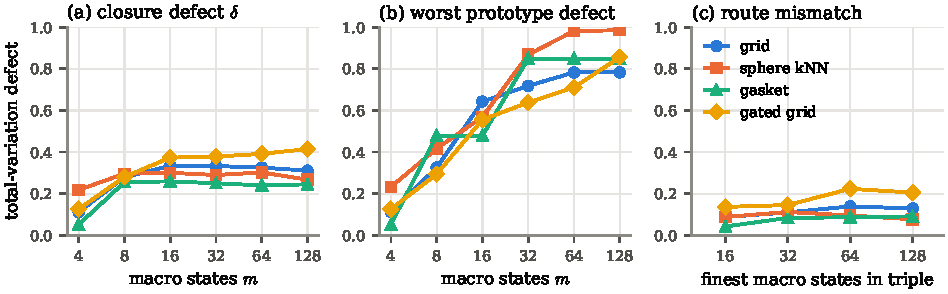
\includegraphics[width=\linewidth]{figures/fig_learned_audit.pdf}
\caption{Audits of the learned ladders at each level. (a) For $m\ge8$ the closure defect $\delta$ remains substantial, between $0.24$ and $0.42$. (b) The worst prototype defect never decreases with resolution (it plateaus at some levels) and reaches $0.78$--$0.99$ at the finest level. (c) Route mismatch on fine prototype inputs, for each nested triple, indexed by its finest level. All values are total-variation distances in $[0,1]$.}
\label{fig:learned-audit}
\end{figure}

\begin{table}[t]
\centering
\small
\caption{Learned ladders at the finest level ($m=128$, $\tau=5$). $\delta$: closure defect; $\bar s$, $\max s$: mean and worst prototype defect; $\RM$: largest route mismatch over nested triples; Dist: largest fitted raw distortion over adjacent levels (cost units); $\bar d$: mean finite off-diagonal distance; $n_\infty$: number of infinite distances. Floating computation.}
\label{tab:learned}
\begin{tabular}{@{}lrrrrrrrr@{}}
\toprule
Substrate & states & $\delta$ & $\bar s$ & $\max s$ & $\RM$ & Dist & $\bar d$ & $n_\infty$ \\
\midrule
Grid & 625 & 0.311 & 0.625 & 0.783 & 0.139 & 6.05 & 13.29 & 0 \\
Sphere $k$NN & 500 & 0.267 & 0.855 & 0.985 & 0.112 & 5.27 & 9.00 & 0 \\
Gasket & 366 & 0.245 & 0.641 & 0.849 & 0.091 & 8.35 & 19.37 & 0 \\
Gated grid & 625 & 0.415 & 0.615 & 0.856 & 0.223 & 11.25 & 13.42 & 0 \\
\bottomrule
\end{tabular}
\end{table}

\Cref{fig:learned-audit,tab:learned} report the audits.
Every macro graph is connected and every distance finite, so each level carries a genuine finite metric.
The closure defect, however, stays between roughly a quarter and two fifths at all but the coarsest levels, and the worst prototype defect never decreases as the resolution increases.
At the finest level a walker started from the worst block's prototype leaves the block with probability $0.78$ on the grid, $0.85$ on the gasket and $0.99$ on the sphere.
These blocks contain only three to five microstates on average, which is small compared with the spread of a five-step walk.
In the terms of \cref{def:coherence}, these ladders do not provide coherent layers at their fine levels; their finite metrics are measurements, not evidence of a stable emergent geometry.

\subsection{Reweighting prototypes cannot repair persistence}

One might hope to lower the defects by choosing better prototypes for the same partition.
For persistence, the best possible choice can be computed exactly.

\begin{theorem}[Optimal prototypes for a fixed partition]
\label{thm:prototype-obstruction}
Fix $P$, $\tau$ and a partition with coarse matrix $C$, and let $B=P^{\tau}C$.
Over all stochastic prototype matrices $U$ supported on the fibres,
\begin{equation}
\min_U\ \max_{x}\ s_U(x)\;=\;\max_x\Bigl(1-\max_{z\in f^{-1}(x)}B_{zx}\Bigr),
\end{equation}
and the minimum is attained by point-mass prototypes.
\end{theorem}

\begin{proof}
By \cref{prop:closure-basic}(iii), $s_U(x)=1-(UB)_{xx}=1-\sum_{z\in f^{-1}(x)}u_x(z)B_{zx}$.
The sum is a convex average of the return probabilities $B_{zx}$ over the fibre, so it is at most their maximum, which a point mass at a maximizing microstate attains.
The fibres are disjoint, so these choices can be made independently.
\end{proof}

\provenance{Lean: \lean{macro_return_le_fiber_bound} and \lean{prototype_defect_ge_fiber_escape} in \lean{PrototypeObstruction.lean} give the lower bound; attainment is the elementary construction above. Exact computation: the canonical values below are rebuilt from the recorded partitions by integer recurrence.}

For the canonical finest partitions the right-hand side is computed exactly from integer five-step recurrences (common denominators $24^5$ for the open grid and $8^5$ for the gasket).
On the grid it equals $6411/8192\approx0.7826$, attained on a two-state fibre whose states both return with probability $1781/8192$; on the gasket it equals $6957/8192\approx0.8492$, attained on a singleton fibre.
Uniform prototypes already achieve these minima, so no reweighting can lower the worst grid or gasket defect.
The result is conditional on the recorded partitions (it does not certify the eigensolver that produced them) and concerns persistence only; it is not a lower bound on $\delta$.
For the sphere the reported $0.985$ refers to uniform prototypes.
With the kernel, the stage $\tau=5$ and the persistence criterion held fixed, persistence can only be restored by changing the lens, and \cref{sec:constructed} does so.

\subsection{Constraints deform the metric at a fixed lens}
\label{sec:anisotropy}

Constraints change which moves are feasible, and so they should change the geometry.
Comparing the canonical grid and gated-grid runs confounds two effects, because the learned partition changes too.
To isolate the dynamical effect we hold the finest canonical grid lens and its prototypes fixed and replace only the micro kernel by its gated version.
The largest change in a macro transition probability is then $0.231$ and the largest change in a macro distance is $2.42$.
For pairs of microstates four lattice steps apart, the ratio of mean horizontal to mean vertical macro distance moves from $0.984$ without gating to $1.087$ with it.
The induced metric is thus deformed by the constraint at a fixed interface.
The horizontal and vertical directions here are readouts supplied by the known substrate, used only to describe the deformation.

\subsection{Local obstructions to Euclidean embedding}
\label{sec:nonembedding}

Is a learned metric locally Euclidean?
A reconstruction algorithm that fits poorly does not answer this, because a different algorithm might fit better.
A certificate must rule out every fit.
For four points in any real inner-product space,
\begin{equation}
d_{01}^2+d_{23}^2\;\le\;d_{02}^2+d_{03}^2+d_{12}^2+d_{13}^2,
\label{eq:quadrilateral}
\end{equation}
because the difference of the two sides is $\|p_0+p_1-p_2-p_3\|^2$.
If certified lower bounds on the ``diagonals'' $d_{01},d_{23}$ and upper bounds on the four ``sides'' violate~\eqref{eq:quadrilateral} even after every distance is perturbed by $\epsilon$, then no embedding of the four points into any inner-product space, of any dimension, reproduces all six distances to within $\epsilon$.

\provenance{Lean: \lean{hilbert_quadrilateral} and \lean{no_hilbert_uniform_approximation} in \lean{EuclideanObstruction.lean}. Exact computation: macro probabilities are rebuilt in integer arithmetic from the recorded partitions, shortest paths are found by exact multiplicative search, and logarithms are enclosed in rational intervals.}

Applied to a neighbourhood of a centre and its $24$ nearest macro neighbours, this yields exact witnesses for the canonical learned metrics: no inner-product fit of the selected gasket patch is accurate to within $9.1\%$ of the patch radius, and none of the grid patch to within $5.6\%$.
Similar witnesses hold for a family of substrate sizes in which a single learned partition with $m=\min(256,\max(16,\lfloor n/3\rfloor))$ macro states is used (grids of $49,121,361,1089$ states with $m=16,40,120,256$, and gaskets of $42,123,366,1095$ states with $m=16,41,122,256$; patches have $\min(24,m-1)$ neighbours): the excluded relative errors are $6.2$--$8.6\%$ for grids and $9.4$--$11.3\%$ for gaskets. For the smallest sizes the patch covers most of the macro graph, so these are global rather than local statements.
The essential point is that the grid fails as well.
Failure of local Hilbert embeddability in a finite learned metric does not by itself indicate a fractal; it is equally a feature of the $L^1$-like metrics that grid walks produce (\cref{sec:grid}).

\subsection{Dimension proxies}

Two finite proxies for dimension are standard: the slope of the logarithm of mean ball size against the logarithm of the radius in the induced metric (ball growth), and the slope of the packaged entropy against the logarithm of the inverse typical spacing across the ladder (information dimension)~\cite{Renyi1959DimensionEntropy,CoverThomas2006,Falconer2003Fractal}.
On a $20\times20$ grid and the level-5 gasket with the canonical ladder, the ball-growth slopes are $1.67$ and $1.39$ and the information slopes $4.66$ and $2.07$.
Replacing the distance $d$ by $\sqrt d$ roughly doubles the ball-growth slopes ($3.34$ and $2.78$), so these numbers depend on the cost convention and cannot be identified with the dimensions $2$ and $\log3/\log2\approx1.585$.
In the size family above (single partition, $m=\min(256,\max(16,\lfloor n/3\rfloor))$), the grid ball-growth slope stays between $1.61$ and $1.77$ and the gasket slope between $1.28$ and $1.38$; the contrast persists, but it is not a dimension estimate.
An exact dimension requires a limit object, which \cref{sec:gasket} constructs.

\section{Three coherent regimes}
\label{sec:constructed}

The learned ladders fail persistence because their blocks are small compared with the distance a walker travels in $\tau$ steps.
This section shows that the failure is a property of those lenses, not of the program.
For three systems we write down nested lenses, explicit floors and explicit distance units, and prove that every requirement of \cref{def:coherence} holds in a joint limit in which substrate and lens are refined together.
The stage is $\tau=5$ throughout.
For the grid and the gasket the micro dynamics is exactly the lazy walk of \cref{sec:learned}; for the sphere it is a new family of reservoir chains.
In all three cases the lens is supplied by the structure of the substrate.
The results therefore establish that coherent geometric layers exist under these dynamics, and identify their limits; they do not show that such lenses can be found from an unlabelled kernel.

All three constructions rest on one mechanism.
\Cref{prop:closure-basic}(iii)--(iv) reduces closure and persistence to escape probabilities, and escape from a large block is rare because a walker must first reach the block boundary.
A probability floor below every positive macro weight leaves all edge costs untouched, and two-sided bounds on macro transition probabilities turn into two-sided bounds on the path metric.
\Cref{fig:defects-vs-cell} contrasts the resulting defects with those of the learned ladders.

\begin{figure}[t]
\centering
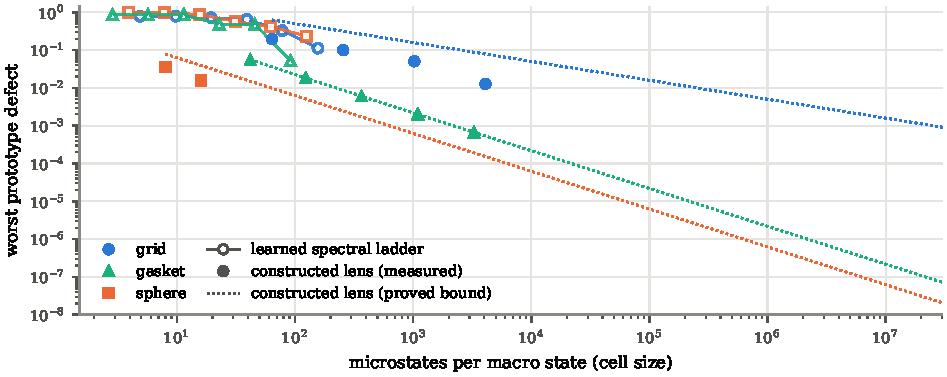
\includegraphics[width=\linewidth]{figures/fig_defects_vs_cell.pdf}
\caption{Worst prototype defect against block size. Hollow markers: the learned spectral ladders of \cref{sec:learned} (one marker per level). Filled markers: measured finite audits of the supplied lenses of this section. Dotted lines: the proved bounds $5/b$ (grid, block size $b^2$), $3\kappa/(V_s-3)$ (gasket, cell size $V_s$) and $5/(8V)$ (spherical reservoirs of volume $V$). For the reservoirs only the finest lens level is shown, where each macro state is a single reservoir and the cell size equals $V$.}
\label{fig:defects-vs-cell}
\end{figure}

\subsection{Grid: block lenses and an \texorpdfstring{$L^1$}{L1} limit}
\label{sec:grid}

Let the micro dynamics be the lazy walk on the open $N\times N$ grid of \cref{sec:substrates}, with $N=Mb$.
The block lens with width $b$ labels the site $(r,c)$ by $(\lfloor r/b\rfloor,\lfloor c/b\rfloor)$, giving an $M\times M$ array of blocks, and each prototype is uniform on its $b\times b$ block.
Lenses whose widths differ by an integer factor are nested by block containment.
Write $L(x,y)$ for the Manhattan distance between block indices.

\begin{theorem}[Coherent block lenses at stage five]
\label{thm:grid}
Let $b\ge8$ and $\tau=5$.
\begin{enumerate}[label=(\roman*)]
\item Every block has escape probability at most $5/b$; hence $\delta\le5/b$ and $\max_x s(x)\le5/b$.
\item Transitions between distinct blocks occur only between blocks that share a side (``cardinal'') or a corner (``diagonal''), with symmetrized weights
$\frac{1}{128b}\le W\le\frac5b$ on cardinal pairs and $\frac{1}{512b^2}\le W\le\frac{25}{b^2}$ on diagonal pairs.
\item With floor $\eta_b=1/(1024b^2)$ and threshold $0$, no edge is clipped, the macro graph is connected, and with $c_b=\log(128b)$ and $e=\log 640$,
\begin{equation}
(c_b-e)\,L(x,y)\;\le\;d_b(x,y)\;\le\;c_b\,L(x,y)\qquad\text{for all }x,y.
\end{equation}
\item In the declared unit $\lambda=Mc_b$, the normalized metric $\rho_b=d_b/(Mc_b)$ satisfies
$\max_{x,y}|\rho_b(x,y)-L(x,y)/M|\le 2\log640/\log(128b)$.
\item For nested lenses with widths $b_{\mathrm f}$ and $b_{\mathrm c}=2b_{\mathrm f}$, the normalized distortion is at most $2/M_{\mathrm f}+2\log640/\log(128b_{\mathrm f})+2\log640/\log(128b_{\mathrm c})$.
\item For a nested triple, the route mismatch on fine prototype inputs is at most $15/b_{\mathrm f}+5/b_{\mathrm m}$.
\end{enumerate}
\end{theorem}

\provenance{Written proof (\cref{app:grid-proof}). Lean: the step from escape to the closure defect on every microstate is \lean{closure_defect_le_macro_escape}. Exact and floating computation: complete ladders on grids of side $64$ and $128$ (finest $256$ blocks) check every macro edge against (ii) and every macro pair against (iii)--(v); tests compare the sparse staged computation with the dense original kernel.}

The escape bound comes from stationarity.
The stationary law of the open grid walk is proportional to vertex degree, a uniform block prototype is pointwise at most a fixed multiple of it, and this domination is preserved by the dynamics.
Each step therefore crosses the block boundary with probability at most $1/b$, and a union bound over five steps gives (i).
For (ii), a five-step walk with $b\ge8$ moves at most one block in each coordinate; explicit paths give the lower bounds and the need to start within five sites of the boundary gives the upper bounds.
The key consequence is (iii): a cardinal step costs about $\log b$ and a diagonal step about $2\log b$, so a cheapest protocol counts Manhattan steps.

\paragraph{Joint refinement and the limit.}
For $k\ge3$ put $t=2^k$, $N=4t^2$, and use the three nested lenses of widths $4t,2t,t$ (block arrays of side $t,2t,4t$).
Every requirement of \cref{def:coherence} holds: closure and prototype defects are at most $5/t$, every macro graph is connected, adjacent normalized distortions and route mismatches tend to zero, the number of blocks grows, and by (iii) the normalized diameter lies between $(1-e/c_b)\,2(M-1)/M$ and $2(M-1)/M$, so it tends to $2$.
Mapping each block to its centre in $[0,1]^2$ turns $L/M$ into exactly the $L^1$ distance between centres, and the centres form a net whose mesh tends to zero.
The normalized macro metrics therefore converge, uniformly on block centres and in the Gromov--Hausdorff sense~\cite{Gromov1999Metric}, to the unit square with the $L^1$ metric; quantitatively, the Gromov--Hausdorff distance is at most $\log640/\log(128b)+1/M$.

Two qualifications are part of the result.
First, the limit is not Euclidean.
The four corners of an $L^1$ square have side lengths $1$ and diagonals $2$, which violates~\eqref{eq:quadrilateral}; so coherence does not imply an inner-product geometry, and failure of Euclidean fit does not indicate a fractal.
Second, the convergence is slow and the units matter.
The readout error in (iv) decays only like $1/\log b$, and it is a conservative bound that is uninformative at the audited block widths, where the measured normalized readout errors are between $0.44$ and $1.06$ and the measured normalized distortions between $0.14$ and $0.30$.
In raw cost units, with the prescribed unit ratio, the distortion is multiplied by the fine unit $M_{\mathrm f}c_{b_{\mathrm f}}$ and need not vanish at all.

\subsection{Gasket: recursive cells and a fractal limit}
\label{sec:gasket}

\begin{figure}[t]
\centering
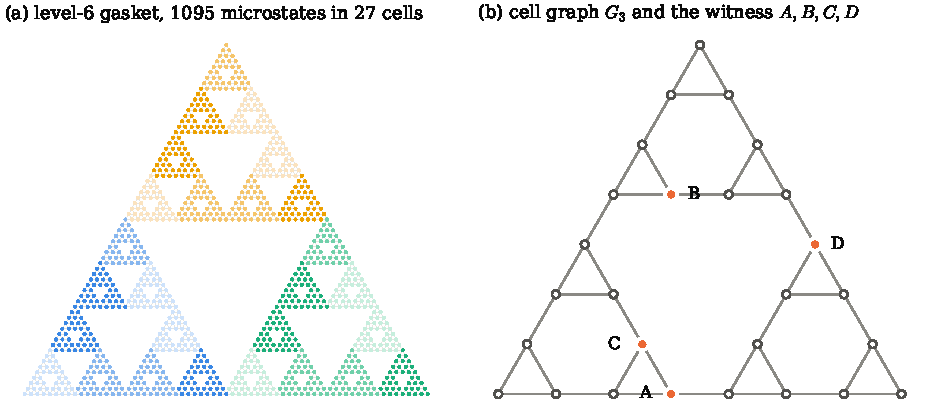
\includegraphics[width=\linewidth]{figures/fig_gasket_cells.pdf}
\caption{(a) The level-6 gasket graph ($1095$ microstates) partitioned into the $27$ recursive cells of level $3$; colours indicate cells (shades group them by their first address digit). (b) The cell contact graph $G_3$, whose unit-edge metric controls the macro metric. The four highlighted cells are the depth-3 prefixes of the limiting points $A,B,C,D$ of \cref{thm:gasket-limit}; their graph distances are $AB=CD=5$, $AC=1$, $BD=3$, $AD=BC=4$.}
\label{fig:gasket-cells}
\end{figure}

Let the micro dynamics be the lazy walk on the level-$\ell$ gasket graph, $\ell=s+m$ with $s\ge3$.
The recursive construction covers this graph by $3^m$ copies of the level-$s$ gasket, each with $V_s=(3^{s+1}+3)/2$ vertices; neighbouring copies share one corner vertex.
Assigning each shared vertex to the lexicographically first copy containing it gives disjoint fibres of sizes between $V_s-3$ and $V_s$, labelled by addresses of length $m$ over $\{0,1,2\}$ (\cref{fig:gasket-cells}a).
The ownership rule is nested, so deleting the last address digit is the containment map to the next coarser lens.
Prototypes are uniform on fibres.
Two cells are adjacent when their copies share a corner; the resulting cell contact graph $G_m$ consists of three copies of $G_{m-1}$ joined pairwise by single edges (\cref{fig:gasket-cells}b).
Let $D_m$ be its unit-edge graph metric.

\begin{theorem}[Coherent recursive cells at stage five]
\label{thm:gasket}
Let $s\ge3$, $m\ge1$, $\tau=5$ and $\kappa=11905/16384$.
\begin{enumerate}[label=(\roman*)]
\item For adjacent cells $K_{xy}=\kappa/n_x$, where $n_x$ is the fibre size; all other off-diagonal entries vanish.
\item Every escape probability, and hence $\delta$ and $\max_x s(x)$, is at most $3\kappa/(V_s-3)$.
\item With floor $\eta_s=\kappa/(2V_s)$ and threshold $0$, no edge is clipped, the macro graph is connected, and with $c_s=\log(V_s/\kappa)$ and $e_s=\log(V_s/(V_s-3))$,
$(c_s-e_s)D_m\le d_{s,m}\le c_sD_m$.
\item In the declared unit $2^mc_s$, the normalized metric $\rho_{s,m}=d_{s,m}/(2^mc_s)$ satisfies $\max|\rho_{s,m}-D_m/2^m|\le\epsilon_s\coloneqq e_s/c_s$.
\item Adjacent lenses on the same micro graph have parameters $(s,m)$ and $(s+1,m-1)$, and their normalized distortion is at most $2^{-m}+\epsilon_s+\epsilon_{s+1}$.
\item For a nested triple with fine and middle cell sizes $V_{\mathrm f}=V_s$ and $V_{\mathrm m}=V_{s+1}$, the route mismatch on fine prototype inputs is at most $\frac{32}{4(V_{\mathrm f}-3)-2}+\frac{3\kappa}{V_{\mathrm f}-3}+\frac{3\kappa}{V_{\mathrm m}-3}$.
\end{enumerate}
\end{theorem}

\provenance{Written proof (\cref{app:gasket-proof}). Exact computation: the interface constant $\kappa$ is the five-step crossing count $23810/8^5$ on the level-4 graph, and the contributing radius-five neighbourhood is the same for every $s\ge3$. Lean: \lean{closure_defect_le_macro_escape} (closure from escape) and \lean{gasket_staged_log_bracket} (cost bracket estimates). Exact and floating computation: complete ladders on gaskets of levels $6$, $7$ and $9$ (up to $29526$ microstates) check every bound; the worst finest prototype defects are $0.054$, $0.018$ and $0.0060$, and the route mismatches $0.0060$, $0.0020$ and $0.00066$.}

Statement (i) is the heart of the construction: since cell corners are at least $2^s\ge8$ steps apart, a five-step walk crosses at most one interface, and the probability flux across an interface is a universal constant independent of $s$.
For three-level ladders $(s+2,m-2)$, $(s+1,m-1)$, $(s,m)$ with $s,m\to\infty$, every requirement of \cref{def:coherence} holds: the number of cells grows and normalized diameters tend to one.

\paragraph{The limit space.}
Represent points by infinite addresses $a\in\{0,1,2\}^{\N}$ and put
\[
\delta_m(a,b)=D_m(a|_m,b|_m)/2^m,
\]
where $a|_m$ is the length-$m$ prefix.
Under last-digit deletion $r$ the graphs satisfy $|D_m(x,y)-2D_{m-1}(r(x),r(y))|\le1$, so $|\delta_{m+1}-\delta_m|\le2^{-(m+1)}$ and the $\delta_m$ converge uniformly.

\begin{theorem}[The gasket limit]
\label{thm:gasket-limit}
The limit $\delta=\lim\delta_m$ is a pseudometric on addresses with $|\delta-\delta_m|\le2^{-m}$. Identifying addresses at distance zero gives a compact metric space $(\mathcal G,\delta)$ of diameter $1$ with the following properties.
\begin{enumerate}[label=(\roman*)]
\item \emph{Self-similarity.} Prefixing a fixed word of length $j$ scales all distances by exactly $2^{-j}$, so $\mathcal G$ is covered by $3^j$ copies of itself scaled by $2^{-j}$.
\item \emph{Convergence of the Markov metrics.} For any $s_m\ge3$ with $s_m\to\infty$, the normalized metrics of \cref{thm:gasket} on micro level $s_m+m$ satisfy $|\rho_{s_m,m}-\delta|\le\epsilon_{s_m}+2^{-m}\to0$ on cell addresses.
\item \emph{Dimension.} With $d_f=\log3/\log2$ and $\mu$ the image of the uniform product measure, every ball satisfies $\tfrac13 r^{d_f}\le\mu(B_x(r))\le10\,r^{d_f}$ for $0<r<1$. Consequently $\dH\mathcal G=\log 3/\log 2$.
\item \emph{No local Hilbert approximation.} For every point $x$ and every $j\ge0$, there is no map from the ball $B_x(2^{-j})$ into a real inner-product space that changes all pairwise distances by at most $2^{-j}/16$.
\end{enumerate}
\end{theorem}

\provenance{Written proof (\cref{app:gasket-proof}), including the recursive graph laws, compactness, the measure bounds and the Hausdorff dimension argument. Lean: the strict scalar inequality behind (iv) is \lean{gasket_limit_quadrilateral_gap}, applied through \lean{no_hilbert_uniform_approximation}. Exact computation: the prefix distance formulas used in (iv) are checked for prefixes of length $3$ to $6$.}

Part (iv) uses four explicit points,
\begin{equation}
A=0\,1^{\infty},\qquad B=20\,1^{\infty},\qquad C=01\,2^{\infty},\qquad D=1\,2^{\infty},
\end{equation}
whose limiting distances are $\delta(A,B)=\delta(C,D)=\tfrac34$, $\delta(A,C)=\delta(B,D)=\tfrac14$ and $\delta(A,D)=\delta(B,C)=\tfrac12$.
These violate the quadrilateral inequality~\eqref{eq:quadrilateral}, and they still violate it with a strict gap of $15/128$ after every distance is moved by $1/16$ in the unfavourable direction.
By self-similarity, the prefix copy of length $j$ containing any given point $x$ lies in $B_x(2^{-j})$ and contains a copy of this configuration scaled by $2^{-j}$.
The finite Markov metrics carry the same obstruction: for $m\ge2$, a fixed six-cycle of $G_2$ remains isometrically embedded in $G_m$, and with the cost bracket of \cref{thm:gasket}(iii) its four-point witness excludes Hilbert fits to within one twelfth of its radius bound $3c_s$ (\lean{gasket_quadrilateral_gap}).
Because the finite witness and the limit approximation error are of comparable size, the limiting statement is proved from the fixed limiting points rather than transferred from finite witnesses.

The gasket limit is thus a genuinely fractal geometry obtained from the original micro dynamics: compact, self-similar, of non-integer Hausdorff dimension, and quantitatively non-Euclidean at every point and every dyadic scale.
It is a different object from the learned gasket ladder of \cref{sec:learned}, which still fails persistence, and the dimension proxies reported there are not estimates of $\log3/\log2$.

\subsection{Sphere: reservoir chains and a curved limit}
\label{sec:sphere}

The sphere $k$NN walk of \cref{sec:learned} has no natural nested lens, so the curved construction changes the micro dynamics.
Each macro point is a \emph{reservoir}: a cycle of $V\ge4$ microstates that holds with probability $5/8$ and moves to each cycle neighbour with probability $3/16$.
One state of each reservoir is its \emph{gateway}.
Given distinct points $q_1,\dots,q_n$ on the unit sphere with geodesic distance $d_S$, and a contact parameter $\beta>0$, gateways $i\neq k$ are linked with probability
\begin{equation}
Q_{ik}=\frac{2^{-\lceil\beta\, d_S(q_i,q_k)\rceil}}{8n},
\end{equation}
and each gateway's holding probability is reduced by its total contact rate.
In matrix form $P=I_n\otimes B+(Q-\operatorname{diag}(Q\one))\otimes G$, where $B$ is the cycle kernel and $G$ projects onto the gateway.
$P$ is stochastic, symmetric and connected, every diagonal entry is at least $\tfrac12$, and the stationary law is uniform.
The spherical geometry enters through the contact law: the substrate is designed to be spherical, just as the grid and gasket substrates are designed to be flat and self-similar.

The points $q_i$ come from nested cube meshes.
Each face of the cube $[-1,1]^3$ is divided into $2^{\ell}\times2^{\ell}$ cells, cell centres are projected radially to the sphere, and in one cell per face the representative is replaced by the face's axis point, so that the six axis points (and three mutually orthogonal ``landmarks'') belong to every mesh.
Dyadic parents give nested lenses.
For $r\ge5$, the system $\mathcal S_r$ has one reservoir per cell of level $r+2$ and lenses at levels $r$, $r+1$ and $r+2$, with
\begin{equation}
n_r=6\cdot4^{r+2},\qquad V_r=2^r,\qquad \beta_r=2^{r/2},\qquad t_r=\beta_r\log2,\qquad\tau=5.
\end{equation}
Every coarse fibre is a union of at most $16$ reservoirs, and prototypes are uniform on fibres.
Distances are measured in the declared unit $t_r$.

\begin{theorem}[Coherent spherical reservoirs]
\label{thm:sphere}
For every $r\ge5$, at all three lens levels of $\mathcal S_r$:
\begin{enumerate}[label=(\roman*)]
\item escape, $\delta$ and $\max_x s(x)$ are at most $5/(8V_r)$;
\item with threshold $0$ and the inactive floor $\eta=2^{-\lceil\beta_r\pi\rceil}/(256\,n_rV_r\cdot16)$, the macro graph is connected and, writing $r_x$ for the representative point of macro state $x$,
\begin{equation}
0\;\le\;\frac{d(x,y)}{t_r}-d_S(r_x,r_y)\;\le\;\epsilon_r\coloneqq 4\pi\sqrt2\,2^{-r}+\bigl(16+\log_2 6+3r\bigr)2^{-r/2};
\end{equation}
\item the normalized distortion between adjacent lens levels is at most $2\epsilon_r+2\varrho_r$, where $\varrho_r=2\pi\sqrt2\,2^{-r}$ bounds the cell radius;
\item the route mismatch is at most $5/(2V_r)$ on fine prototype inputs and at most $15a_r+5/(8V_r)$ on every micro point mass, where $a_r=O(2^{-r})$ bounds the contact rate of any gateway;
\item the normalized macro spaces converge in the Gromov--Hausdorff sense to the unit sphere with its geodesic metric; their diameters lie in $[\pi,\pi+\epsilon_r]$.
\end{enumerate}
\end{theorem}

\provenance{Written proof (\cref{app:sphere-proof}): killed-walk density bounds, first-contact flux with exponential moments, a per-edge baseline inequality, cube-mesh covering and packing estimates. Lean: \lean{likelihood_cost_exp_bracket}, \lean{Protocol.reference_le_cost} and \lean{weightedEdist_reference_bracket} in \lean{CoherentMetric.lean} pass probability brackets to the actual floored costs and to the protocol infimum; \lean{closure_defect_le_macro_escape} gives (i). Exact computation: at the finest lens (one reservoir per macro state) the stage-five macro kernel is $K_5=I+\frac1V\sum_{k=1}^5c_kA^k$ with $c=(5,\tfrac{7345}{1024},\tfrac{109}{16},\tfrac{31}{8},1)$ and $A=Q-\operatorname{diag}(Q\one)$, for every $V\ge4$; coarser kernels follow by uniform lifting and aggregation. Floating computation: two finite reservoir ladders with $768$ and $6144$ microstates, using smaller parameters than the family $\mathcal S_r$ (whose first member already has $3{,}145{,}728$ microstates), check the general finite-reservoir bounds under those parameters.}

The proof of (ii) is the delicate step.
An upper bound on $K_{xy}$ must allow walks that make several contacts, possibly back and forth, within five steps; this is handled by an exponential moment of the displacement, which grows by at most a factor $9/8$ per step.
A lower bound comes from a single contact followed by four holds.
Together they give, for every off-diagonal pair, $t\,d_S(r_x,r_y)\le c(x,y)\le t\,d_S(r_x,r_y)+2t\varrho_r+\log(256\,n_rV_r\cdot16)$; the additive term grows only linearly in $r$, so it is $o(t_r)$ and vanishes after division by the unit $t_r$. The lower bound holds for each edge separately, so coarsening errors cannot accumulate along long protocols.
Route coherence from every microstate, not just from prototypes, needs a packing estimate: no gateway has many reservoirs nearby, so the contact rate $a_r$ from any single microstate is small.

The construction keeps the stage, the likelihood cost, the shortest-path readout and all coherence gates, and changes the micro dynamics and the lens family; we do not claim that these changes are necessary.
Its parameters are tuned to the limit: the finite audits use small volumes and contact parameters outside the family $\mathcal S_r$, at which the metric error bound is far from small, so they check the implementation rather than illustrate convergence.
The limits involve probabilities of order $2^{-\beta_r\pi}$, which double-precision arithmetic cannot represent for large $r$; the family is a mathematical construction, not a scalable simulation.
\Cref{sec:transport-repair} shows that its metrics carry enough information to recover spherical curvature.

\section{Curvature as route dependence of transport}
\label{sec:curvature}

Coherence of distances does not reveal curvature: a sphere and a plane can both carry perfectly coherent metrics.
Curvature appears when one \emph{transports} something, say a frame, along different routes between the same endpoints and compares the results~\cite{Lee1997Riemannian}.
This section makes that idea precise for discrete transports, tests the local-MDS estimator used in our pipeline against it, and shows how curvature can be recovered from the Markov metrics of \cref{sec:sphere}.

\subsection{Holonomy is noncommutation of covariant shifts}
\label{sec:connection}

A tempting slogan is that curvature is ``noncommutativity of local moves''.
Taken literally for planar frames it is false: two rotations of the plane always commute, because $SO(2)$ is abelian.
The correct statement involves operators that move the base point as well as the frame.

Let $X$ carry two commuting translations $u$ and $v$ (for example the two directions of a periodic grid), and suppose each $x\in X$ has a two-dimensional fibre with an orthonormal frame.
Let $A_x$ and $B_x$ be orthogonal matrices transporting the fibres at $ux$ and $vx$ back to $x$.
On the space of sections $s$ (one vector per fibre) define the \emph{covariant shifts}
\begin{equation}
(S_us)(x)=A_x\,s(ux),\qquad (S_vs)(x)=B_x\,s(vx).
\end{equation}
The two routes from $uvx$ back to $x$ have transports $L_x=A_xB_{ux}$ and $M_x=B_xA_{vx}$, and their discrepancy is the square holonomy $H_x=L_xM_x^{-1}$.

\begin{theorem}[Holonomy as a commutator]
\label{thm:commutator}
$\bigl([S_u,S_v]s\bigr)(x)=(H_x-I)\,M_x\,s(uvx)$ for every section $s$.
Hence $S_u$ and $S_v$ commute if and only if $H_x=I$ for every $x$.
If $X$ is finite (so $u,v$ are permutations) and sections carry the $\ell^2$ norm, then $\|[S_u,S_v]\|=\max_x\|H_x-I\|$; if moreover every $H_x$ is a rotation, with angle $\theta_x\in[0,\pi]$, this equals $\max_x 2\sin(\theta_x/2)$ (an orientation-reversing $H_x$ has $\|H_x-I\|=2$ and no rotation angle).
Under independent frame changes $Q_x\in O(2)$, $H_x\mapsto Q_xH_xQ_x^{-1}$ and the commutator is conjugated by an orthogonal map, so $\theta_x$ and the norm are invariant.
\end{theorem}

\provenance{Lean: \lean{covariantShift_commute_iff}, \lean{covariantShift_gauge} and \lean{plaquetteHolonomy_gauge} in \lean{Connection.lean}, for group-valued frame fields acting by their regular action, including abelian groups. Written proof: the linear formula, the norm identity and the angle formula (\cref{app:connection-proof}).}

The commutator is nonzero when the coefficients, evaluated at \emph{different} base points, fail to satisfy $A_xB_{ux}=B_xA_{vx}$, which abelian coefficients do not prevent.
Conversely, constant coefficients that commute with each other, for instance constant rotations, give commuting shifts and trivial holonomy even when each individual transport is a nontrivial rotation, so patchwise framing does not by itself create curvature.
For triangular loops the same idea reads: invertible transports $a\colon x\to y$, $b\colon y\to z$, $c\colon x\to z$ satisfy $ab c^{-1}=1$ if and only if $ab=c$ (\lean{triangleHolonomy_eq_one_iff}), and for orthogonal transports whose triangle holonomy is a rotation by $\theta$, the disagreement between the two-step and the direct route is $\|ab-c\|=2\sin(\theta/2)$.

\paragraph{An exact curved example.}
On the unit sphere with latitude $\phi$ and longitude $\lambda$, the Levi-Civita connection in the frame $(e_\phi,e_\lambda)$ transports along a latitude by the rotation $R(\sin\phi\,\Delta\lambda)$ and along a meridian by the identity.
For the rectangle bounded by latitudes $\phi_0<\phi_1$ and a longitude interval of width $w$, the square holonomy is the rotation by $-w(\sin\phi_1-\sin\phi_0)$, minus the enclosed area.
With $\sin\phi_0=\tfrac14$, $\sin\phi_1=\tfrac12$ and $w=\tfrac14$, the area and the holonomy angle are both exactly $1/16$, and $\|[S_u,S_v]\|=2\sin(1/32)>0$; the flat connection gives zero.
For rectangles of side $h$ around a fixed latitude, the principal angle divided by the area equals $1$ whenever the area is below $\pi$, in particular for all small $h$, while the raw angle tends to zero.
Recovering curvature from shrinking loops therefore requires normalizing by area; a raw angle that vanishes under refinement is not evidence of flatness.

\subsection{The local-MDS and Procrustes estimator}
\label{sec:mds-estimator}

Our pipeline estimates holonomy from a finite metric as follows.
Each macro state and its $k$ nearest neighbours (optionally expanded by one hop) are embedded in the plane by classical multidimensional scaling~\cite{BorgGroenen2005}, keeping the two leading positive eigenvalues.
The transport between two overlapping charts is the orthogonal polar factor of the cross-covariance of their centred overlap coordinates, the orthogonal Procrustes solution~\cite{Schonemann1966}, computed over the full group $O(2)$ because each MDS chart is determined only up to rotation \emph{and} reflection.
Overlaps or cross-covariances of deficient rank are excluded.
For a sampled triangle of neighbouring states the holonomy score is the rotation angle of the product of the three transports; orientation-reversing products have no rotation angle and are counted separately.
By \cref{thm:commutator} and the triangle criterion, these scores are gauge invariant and measure the route disagreement of the estimated discrete connection.
For an exact planar Euclidean metric every full-rank chart is an isometric copy of the plane coordinates, and every triangle holonomy is exactly zero.

\begin{figure}[t]
\centering
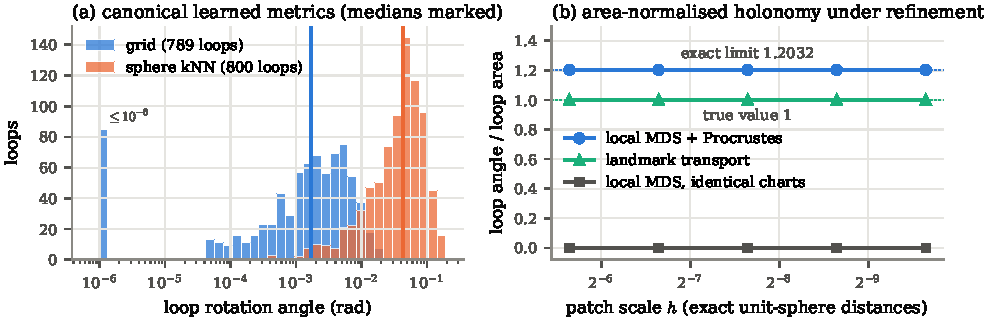
\includegraphics[width=\linewidth]{figures/fig_holonomy.pdf}
\caption{Holonomy estimation. (a) Loop rotation angles on the canonical learned metrics ($m=128$, $\tau=5$; $k=24$ chart neighbours, one-hop expansion, triangles from $8$ nearest neighbours). Medians over all evaluated loops: $0.00169$ (grid) and $0.0428$ (sphere $k$NN). No loop was excluded; the $85$ grid angles below $10^{-6}$ (numerically zero) are collected in the leftmost bin. (b) Exact unit-sphere distances on a fixed $12$-point patch scaled by $h$: the area-normalized output of the local-MDS estimator converges to the exact constant $\approx1.20317$, the same estimator with identical charts returns $0$, and the landmark transport estimator of \cref{sec:transport-repair} returns $1$. Floating computation; the limit constant is exact.}
\label{fig:holonomy}
\end{figure}

\paragraph{Finite separation on the learned metrics.}
On the canonical learned metrics (\cref{fig:holonomy}a), the median triangle angle is $0.00169$ radians on the grid ($789$ triangles) and $0.0428$ on the sphere $k$NN substrate ($800$ triangles), a ratio of about $25$; no triangle was excluded for missing transport or reversed orientation.
The estimator thus separates the two substrates under this fixed protocol.
What it measures is the non-flatness of the estimated connection on two learned metrics that, by \cref{sec:learned}, are not coherent layers.
It is not an estimate of Riemannian curvature, and the next result shows that it could not be one in general.

\begin{theorem}[The local-MDS estimator is not a consistent curvature estimator]
\label{thm:mds-obstruction}
Apply the estimator to exact geodesic distances on the unit sphere, for point configurations obtained by mapping a fixed planar configuration through the exponential map at scale $h\to0$.
\begin{enumerate}[label=(\roman*)]
\item If the three charts of a triangle contain the same point set, their overlaps have full rank, and the second and third eigenvalues of the centred Gram matrix are distinct (which holds for all small $h$), the estimated holonomy is exactly zero. For noncollinear chart centres the enclosed spherical area is positive, so the curvature is missed entirely.
\item For an explicit configuration of $12$ points with $k=8$, the three charts are distinct, every chart and overlap stays uniformly nondegenerate after rescaling coordinates by $1/h$ (cross-covariances by $1/h^2$), and the estimated angle divided by the true spherical area converges to
\begin{equation}
\frac{7884106465972959320549378723}{6552773242191625884795360000}\approx1.20317>\tfrac65 .
\end{equation}
\item Both configurations can be embedded in samples that become dense on the whole sphere without changing the three charts.
\end{enumerate}
\end{theorem}

\provenance{Written proof (\cref{app:mds-proof}): second-order expansion of spherical distances, perturbation of the retained spectral subspace across the gap to the zero eigenvalues, and the first-order polar factor; the limiting constant is computed in exact rational arithmetic. Lean: \lean{triangleHolonomy_common_chart} gives the cancellation in (i). Floating computation: \cref{fig:holonomy}b, $h=2^{-k}/50$ for $k=0,\dots,4$.}

Part (i) holds because identical point sets give the same Gram matrix up to a permutation, so with a strict eigenvalue gap the three charts are gauge copies of one another, whatever the curvature.
Part (ii) shows that the failure is not caused by degenerate charts or reflections: with distinct, well-conditioned charts the bias in the area-normalized output is about $20\%$ in the limit.
The estimator does satisfy a stability bound: for nonsingular cross-covariances $M,N$ with polar factors $U,V$,
$\|U-V\|_F\le2\|M-N\|_F/(\sigma_{\min}(M)+\sigma_{\min}(N))$.
But in charts of size $h$ the coordinate errors induced by curvature are of order $h^3$, which permits transport errors of order $h^2$, exactly the order of curvature times area.
The bound cannot make the area-normalized error vanish, and (ii) shows that it does not.

\subsection{Landmark transport and curvature from Markov metrics}
\label{sec:transport-repair}

If the metric is known to be (close to) that of the unit sphere and three mutually orthogonal landmark points $a_1,a_2,a_3$ are marked, curvature can be recovered consistently.
Each point $i$ is reconstructed as $p_i=r_i/|r_i|$ with $r_i=(\cos d(i,a_1),\cos d(i,a_2),\cos d(i,a_3))$, which recovers its position in the landmark basis exactly for exact spherical distances.
The minimal rotation taking $p$ to $q$,
\begin{equation}
R(p,q)=I+K+\frac{K^2}{1+p\cdot q},\qquad K=\text{the cross-product matrix of }p\times q,
\end{equation}
is parallel transport along the shorter great-circle arc, and tangent frames are obtained by projecting a fixed unit reference vector onto each tangent plane and normalizing.
Around a geodesic triangle of area below $\pi$ the resulting principal loop angle equals the enclosed area, by Stokes' theorem applied to the connection form of the frame.

\begin{theorem}[Quantitative landmark transport]
\label{thm:landmark}
Suppose all measured distances, including those to the landmarks, are within $\epsilon\le1/(2\sqrt3)$ of true unit-sphere distances.
Suppose also that, for both the true and the reconstructed points, the tangential projections of the unit reference vector have length at least $\kappa>0$ and every arc satisfies $1+p\cdot q\ge\gamma>0$.
Then for every geodesic triangle whose true area is below $\pi$
\begin{equation}
\bigl|\text{estimated angle}-\text{true area}\bigr|\;\le\;3\pi\sqrt3\,C\,\epsilon,
\qquad C=4+\frac{16}{\kappa}+\frac4\gamma+\frac2{\gamma^2}.
\end{equation}
\end{theorem}

\provenance{Written proof (\cref{app:landmark-proof}). Lean: \lean{triangle_transport_error} bounds the error of a product of three approximate contractions in a normed ring, and \lean{normalized_angle_error} divides angle error by a positive area.}

Consistency under refinement therefore needs more than metric convergence: the metric error must be small compared with the loop area, $\epsilon/\text{area}\to0$.
The reservoir family of \cref{sec:sphere} supplies exactly this.

\begin{theorem}[Curvature from staged Markov metrics]
\label{thm:markov-curvature}
In the spherical reservoir family, use the normalized metrics $d/t_r$ (values above $\pi$ clipped to $\pi$ for reconstruction only), the three positive axis points as landmarks, and triangles formed by the north landmark and two mesh points at gnomonic coordinates near $(h_r,0)$ and $(0,h_r)$, with $h_r=2^{-r/8}$.
Then the true triangle areas are at least $h_r^2/8$, the margins $\kappa=0.8$ and $\gamma=1.8$ hold for all large $r$, and the landmark estimator satisfies
\begin{equation}
\left|\frac{\text{estimated angle}}{\text{true area}}-1\right|\;\le\;24\pi\sqrt3\,C\,\frac{\epsilon_r}{h_r^2}\;\longrightarrow\;0,
\end{equation}
because $\epsilon_r/h_r^2=4\pi\sqrt2\,2^{-3r/4}+(16+\log_26+3r)\,2^{-r/4}$.
The area-normalized curvature read from the actual staged Markov metrics converges to $1$, the curvature of the unit sphere.
\end{theorem}

\provenance{Written proof (\cref{app:sphere-proof}), combining \cref{thm:sphere}(ii) with \cref{thm:landmark}. Floating computation: three finite end-to-end controls (Markov kernel to metric to transport, reservoir volume $8$, $\beta=64,128,256$, triangle area $\approx0.0196$) give area-normalized angles $1.077$, $1.083$ and $1.033$; these illustrate the pipeline but do not by themselves establish convergence.}

The result uses recognition input that the learned ladders do not provide: the knowledge that the metric is spherical, three marked orthogonal landmarks, and the declared unit $t_r$.
It does not show that an unknown manifold can be recognized from its Markov metric, and it does not reinterpret the finite learned-metric scores above as curvature estimates.
What it does show is that the chain \emph{dynamics $\to$ lens $\to$ likelihood path metric $\to$ transport $\to$ curvature} can be closed with proofs at every link.

\section{Pythagoras as a law of accounting}
\label{sec:pythagoras}

The Pythagorean theorem is usually presented as a fact about Euclidean triangles.
From the accounting point of view it is a statement about costs: if the cost of a displacement is a positive quadratic form, and the two coordinate directions are orthogonal for that form, then the cost of a diagonal displacement is the sum of the costs of its two legs.
This section shows that staging an isotropic walk produces exactly this situation, with uniform error bounds, and that a matched walk with correlated steps produces a quadratic cost for which the coordinate axes are not orthogonal.

The setting differs from that of \cref{sec:constructed}.
There is no lens: we consider the one-shot cost of a long displacement, not the cheapest chain of macro transitions.
Let $p_n(z)$ be the probability that the lazy walk on $\Z^2$ (stay with probability $\tfrac12$, each cardinal move with probability $\tfrac18$) is displaced by $z$ after $n$ steps.
The \emph{staged cost} is $-\log p_n(z)$, and the \emph{centred cost} is $F_n(z)=\log\bigl(p_n(0)/p_n(z)\bigr)$.

\subsection{A uniform quadratic limit}

\begin{theorem}[Uniform local estimate]
\label{thm:local-limit}
Let $g_n(z)=\frac{2}{\pi n}\exp(-2|z|^2/n)$ and $a=11/96$.
For every $n\ge2$ and every $z\in\Z^2$,
\begin{equation}
|p_n(z)-g_n(z)|\;\le\;B_n\coloneqq\frac{7}{768\pi a^3}\,\frac{n}{(n-1)^3}+\frac{\pi}{2n}e^{-n/(2\pi^2)}+\frac{2}{\pi n}e^{-n/8}.
\end{equation}
\end{theorem}

\provenance{Written proof (\cref{app:quadratic-proof}) from the exact Fourier inversion formula for $p_n$, whose characteristic function $\varphi(t)=\tfrac12+\tfrac14(\cos t_1+\cos t_2)$ takes values in $[0,1]$, together with elementary Taylor and sine bounds and an explicit Gaussian integral. No weak-convergence argument is used.}

The coefficient $2/n$ is not fitted: it is the inverse of twice the per-axis variance $n/4$ of the walk.
Dividing by the explicit lower bound on $g_n$ in a central window gives a relative error, which is what is needed before taking logarithms.

\begin{corollary}[Quadratic accounting and a Euclidean readout]
\label{cor:quadratic}
Fix $R\ge0$ and put
\begin{equation}
E_R(n)=e^{2R^2}\Bigl[\tfrac{4032}{1331}\,\tfrac{n^2}{(n-1)^3}+\tfrac{\pi^2}{4}e^{-n/(2\pi^2)}+e^{-n/8}\Bigr],\qquad d_R(n)=\frac{2E_R(n)}{1-E_R(n)}.
\end{equation}
Whenever $E_R(n)<1$, every $z$ with $|z|\le R\sqrt n$ has $p_n(z)>0$ and $F_n(z)\ge0$, and
\begin{align}
\bigl|F_n(z)-2|z|^2/n\bigr|&\le d_R(n), \label{eq:quad-limit}\\
\bigl|-\log p_n(z)-\log(\pi n/2)-2|z|^2/n\bigr|&\le \frac{E_R(n)}{1-E_R(n)},\\
\bigl|F_n(x,y)-F_n(x,0)-F_n(0,y)\bigr|&\le3\,d_R(n), \label{eq:axis-residual}\\
\Bigl|\sqrt{F_n(z)/2}-|z|/\sqrt n\Bigr|&\le\sqrt{d_R(n)/2}. \label{eq:readout}
\end{align}
Since $E_R(n)=O_R(1/n)$, all four errors tend to zero uniformly on the window.
\end{corollary}

\provenance{Written proof from \cref{thm:local-limit}. Nonnegativity of $F_n$ follows from $p_n(0)-p_n(z)=(2\pi)^{-2}\int\varphi^n(1-\cos t\cdot z)\,dt\ge0$, which uses $\varphi\ge0$. Lean: \lean{abs_log_le_relative_error}, \lean{log_cost_error}, \lean{centered_log_ratio_error}, \lean{cost_axis_residual_bound} (\lean{QuadraticLimit.lean}) and \lean{quadratic_cost_readout_error} (\lean{Pythagoras.lean}) mechanize the passage from relative probability error to the cost, residual and readout bounds.}

Three consequences are worth spelling out.
First, \eqref{eq:quad-limit} says that the staged cost becomes a quadratic form in the displacement, with offset $\log(\pi n/2)$ and coefficient $2/n$ both predicted from the dynamics.
Second, \eqref{eq:axis-residual} says that the cost of a diagonal displacement equals the sum of the costs of its legs, up to a vanishing error: this is the Pythagorean law in cost form.
Third, \eqref{eq:readout} gives a genuine Euclidean geometry.
Let $K$ be a bounded set in the plane, represent $u\in K$ on the lattice by $z_n(u)=(\lfloor\sqrt n\,u_1\rfloor,\lfloor\sqrt n\,u_2\rfloor)$, and choose $R\ge\operatorname{diam}(K)+\sqrt2$, so that every difference $z_n(u)-z_n(v)$ lies in the window $|z|\le R\sqrt n$. Whenever $E_R(n)<1$,
\begin{equation}
\sup_{u,v\in K}\Bigl|\sqrt{F_n\bigl(z_n(u)-z_n(v)\bigr)/2}-|u-v|\Bigr|\;\le\;\sqrt{d_R(n)/2}+\sqrt{2/n}\;\longrightarrow\;0,
\end{equation}
so the square-root readout of the staged cost converges uniformly to Euclidean distance.
The squared cost itself is not a metric (squared distance violates the triangle inequality on the points $0,1,2$ of a line), and the finite readout need not satisfy the triangle inequality exactly; its limit does.

\paragraph{Finite substrates.}
On a torus of side $N$, displacements up to $n$ steps cannot wrap around onto other reachable displacements when $N>2n$, so the torus probabilities coincide with the lattice ones.
This covers the torus of side $512$ used below for all stages up to $128$.
An asymptotic statement on tori requires $N$ to grow with $n$; on a fixed torus the walk eventually becomes uniform and the quadratic law disappears.
For the same reason the theorem uses the true probabilities: a fixed positive probability floor or fitting threshold would eventually discard central probabilities, which are of order $1/n$.

\subsection{Exact certificates and finite runs}

The bounds of \cref{cor:quadratic} are conservative; at the original stages an exact certificate is sharper.
The probabilities are $\mathrm{count}_\tau(z)/8^\tau$ with integer counts computed by exact recurrence. For the six stages $\tau=4,8,16,32,64,128$, on the windows $|x|,|y|\le\lfloor\sqrt\tau\rfloor$, the inequality $|F_\tau(z)-2|z|^2/\tau|\le\delta_\tau$ is verified using rational enclosures of the exponential function.
The certified errors are $\delta_\tau=\tfrac{363}{500},\tfrac{117}{1000},\tfrac{177}{1000},\tfrac{11}{200},\tfrac{11}{250},\tfrac1{50}$ for $\tau=4,8,16,32,64,128$ (windows of $25$ to $529$ points; \cref{fig:quadratic}d).
At $\tau=128$ the readout $\sqrt{F_\tau/2}$ is therefore within $\sqrt{\delta_\tau/2}=0.1$ of $|z|/\sqrt\tau$ on the whole $529$-point window.

\provenance{Exact computation (integer recurrence and rational Taylor enclosures of degree $80$, rebuilt by an independent verifier). Lean: \lean{quadratic_cost_readout_error} turns the certified bound into the readout bound.}

\begin{figure}[t]
\centering
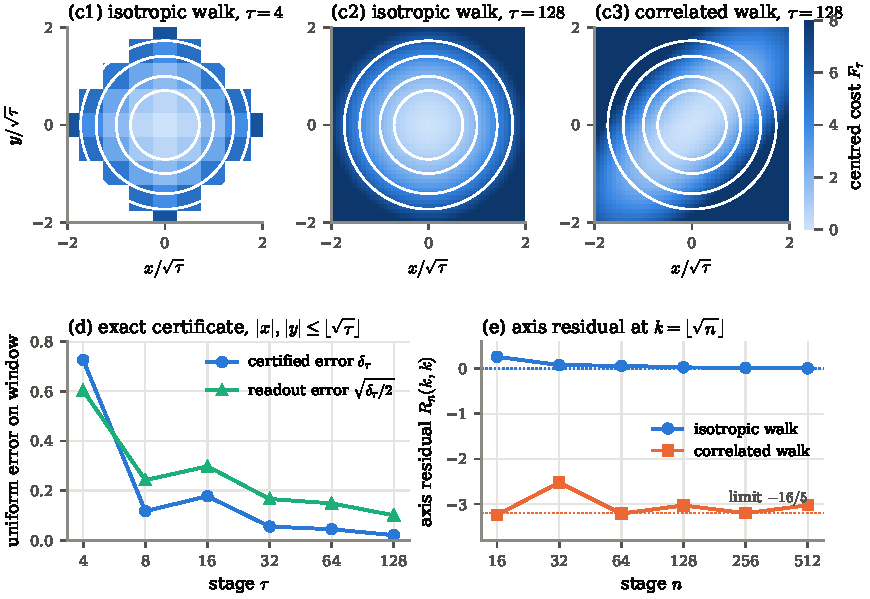
\includegraphics[width=\linewidth]{figures/fig_quadratic.pdf}
\caption{Quadratic accounting. (c1--c3) Centred cost $F_\tau$ in diffusive units $z/\sqrt\tau$; white circles are the level sets $2|z|^2/\tau\in\{1,2,4,6\}$ of the isotropic limit, blank cells are unreachable displacements. At $\tau=4$ the support is a diamond; at $\tau=128$ the isotropic cost is approximately circular, while the correlated walk's cost is approximately elliptical with axes along the diagonals. (d) Exact certificate: uniform centred-cost error $\delta_\tau$ and readout error $\sqrt{\delta_\tau/2}$ on the windows $|x|,|y|\le\lfloor\sqrt\tau\rfloor$. (e) Axis residual $F_n(k,k)-F_n(k,0)-F_n(0,k)$ at $k=\lfloor\sqrt n\rfloor$; the correlated walk's residual equals $-\tfrac{16}5k^2/n$ up to a vanishing error, which oscillates with the rounding of $\sqrt n$ and tends to $-16/5$. Panels (c) and (e): floating computation by nonnegative convolution; panel (d): exact.}
\label{fig:quadratic}
\end{figure}

Floating-point runs on the torus of side $512$ give a consistent picture over larger windows (half-width $\lceil3\sqrt\tau\,\rceil$, capped at $30$), with probabilities computed by nonnegative convolution so that unreachable displacements have probability exactly zero.
A least-squares quadratic fit to the cost has root-mean-square error $0.471$ at $\tau=4$ and $0.151$ at $\tau=128$ ($0.246$ and $0.024$ relative to the spread of the cost), and the median absolute axis residual over $2000$ sampled right triangles drops from $0.862$ to $0.059$.
Neither trend is monotone: as the window grows with $\tau$ the fit error first rises, to $1.19$ at $\tau=32$, before falling.
At $\tau=4$ only $307$ of the $2000$ triangles are supported, so these comparisons are over changing domains and are descriptive only.
Along the axes, a quadratic model fits the cost with error $0.018$ at $\tau=128$, against $1.05$ for a linear model.

\subsection{Controls}

\paragraph{What the residual does and does not test.}
The axis residual~\eqref{eq:axis-residual} tests \emph{separability} of the cost along the coordinate axes, not quadratic shape.
The Manhattan cost $|x|+|y|$ has residual exactly zero, yet its contours are diamonds, its axis profile is linear, and squaring it violates the Pythagorean identity by $2|xy|$.
Quadratic shape is established separately, by~\eqref{eq:quad-limit}, by the certificate, and by the axis fits.

\paragraph{A matched dynamical control.}
Keep the holding probability $\tfrac12$, give each cardinal move probability $\tfrac1{16}$, and add the diagonal moves $(1,1)$ and $(-1,-1)$ with probability $\tfrac18$ each.
The step covariance becomes $\Sigma=\bigl(\begin{smallmatrix}3/8&1/4\\1/4&3/8\end{smallmatrix}\bigr)$, and the same Fourier argument gives a uniform local estimate with the limiting cost
\begin{equation}
Q_n(x,y)=\frac{z^{\mathsf T}\Sigma^{-1}z}{2n}=\frac{12}{5}\,\frac{x^2+y^2}{n}-\frac{16}{5}\,\frac{xy}{n}.
\end{equation}
The cross term makes the axis residual at the diagonal displacement $x=y=\lfloor\sqrt n\rfloor$ tend to $-16/5$ (\cref{fig:quadratic}e); exact certificates at $n=16,32,64,128$ place it strictly below $-1$.
The control does not destroy the Pythagorean law.
$Q_n$ is still a positive quadratic form, and Pythagoras holds for its own inner product; what fails is the orthogonality of the coordinate axes.
Correlation or anisotropy therefore changes \emph{which} directions are orthogonal, and an anisotropic walk with diagonal covariance would keep the coordinate axes orthogonal while turning circles into ellipses.

\provenance{Written proof (Fourier estimate for the correlated walk, \cref{app:quadratic-proof}). Exact computation: integer counts with denominator $16^n$ and rational logarithm enclosures at four stages. Floating computation: \cref{fig:quadratic}e.}

\paragraph{Relation to the macro metric.}
The staged cost is a one-shot account of a single long displacement.
It is not the shortest-path metric of \cref{sec:construction}, and comparing a diagonal cost with the sum of two axis costs at the same $\tau$ is an identity about the shape of the cost, not a statement that a $\tau$-step protocol costs the same as two composed $\tau$-step protocols.
The open-grid walk of \cref{sec:grid} follows the same bulk rule (hold with probability $\tfrac12$, otherwise move to a uniformly chosen neighbour) and differs only at the boundary, where the moving probability is shared among fewer neighbours; under block lenses its path metric converges to the $L^1$ distance.
Both geometries are legitimate readouts of the same local rule; they answer different accounting questions.

\section{Robustness, failure modes and scope}
\label{sec:limits}

\subsection{Sensitivity of the learned pipeline}

Fourteen sensitivity configurations perturb the canonical runs: eleven concern the learned ladders (stage, ladder range, prototypes, edge threshold, holonomy settings) and three concern the staged costs.
\Cref{tab:sweeps} lists the learned-ladder audits; all values are floating computations.

\begin{table}[t]
\centering
\small
\caption{Sensitivity of the learned pipeline: $\delta$ and $\max s$ at the finest level, $\RM$ the largest route mismatch over nested triples. Unless stated, $\tau=5$, levels $4$--$128$, uniform prototypes and $\varepsilon_{\mathrm{edge}}=10^{-15}$.}
\label{tab:sweeps}
\begin{tabular}{@{}llrrrr@{}}
\toprule
Substrate & Change & finest $m$ & $\delta$ & $\max s$ & $\RM$ \\
\midrule
Grid & none (canonical) & 128 & 0.311 & 0.783 & 0.139 \\
Grid & $\tau=1$ & 128 & 0.300 & 0.403 & 0.107 \\
Grid & $\tau=20$ & 128 & 0.278 & 0.939 & 0.134 \\
Grid & levels $4$--$32$ & 32 & 0.324 & 0.508 & 0.125 \\
Grid & levels $8$--$256$ & 256 & 0.307 & 0.869 & 0.154 \\
Grid & stationary-conditional prototypes & 128 & 0.318 & 0.783 & 0.144 \\
Grid & $\varepsilon_{\mathrm{edge}}=0.01$ & 128 & 0.311 & 0.783 & 0.139 \\
Sphere $k$NN & none (canonical) & 128 & 0.267 & 0.985 & 0.112 \\
Sphere $k$NN & $\tau=1$ & 128 & 0.528 & 1.000 & 0.187 \\
Sphere $k$NN & $\tau=30$ & 128 & 0.240 & 0.996 & 0.057 \\
Sphere $k$NN & stationary-conditional prototypes & 128 & 0.269 & 0.985 & 0.105 \\
\bottomrule
\end{tabular}
\end{table}

\paragraph{Stage and resolution.}
On the grid, shorter staging lowers the worst prototype defect ($0.40$ at $\tau=1$) and longer staging raises it ($0.94$ at $\tau=20$); a coarser ladder lowers it and a finer one raises it.
No setting makes it small, which is what \cref{sec:constructed} leads one to expect when blocks contain only a few microstates.
On the sphere $k$NN substrate the worst defect is at least $0.98$ in every sweep.

\paragraph{Prototypes.}
Stationary-conditional prototypes leave the worst grid defect at $0.783$, as \cref{thm:prototype-obstruction} predicts for any prototype choice on this partition.

\paragraph{Connectivity.}
The sweeps named for edge thresholding raise $\varepsilon_{\mathrm{edge}}$ to $0.01$ but remain connected, with no infinite distances; they do not demonstrate a disconnection failure.
Disconnection is nevertheless a real failure mode: the test suite contains a threshold that does disconnect the macro graph, and in that case the global distortion audit fails rather than reporting a discrepancy over the surviving finite pairs.

\paragraph{Holonomy settings.}
Within the sphere pipeline (level $m=64$, $18$ chart neighbours), the median loop angle is $0.083$ over $369$ loops.
A configuration with smaller charts and no expansion ($12$ neighbours, minimum overlap $6$), together with a different loop neighbourhood ($6$ instead of $8$) and loop budget ($800$ instead of $500$), leaves the median similar ($0.086$) but roughly halves the number of evaluable loops ($190$).
Varying the stage moves the median between $0.066$ ($\tau=1$) and $0.106$ ($\tau=30$).
The scores depend on chart parameters, as \cref{thm:mds-obstruction} explains they must.

\paragraph{Staged costs.}
Extending the isotropic stages to $\tau=256$ (stages $16$--$256$) on a torus of side $1024$ continues the trend of \cref{sec:pythagoras} (fit error $0.019$, median residual $0.008$).
On a torus of side $32$ with $\tau$ up to $256$ the window condition $N>2\tau$ fails, yet the residuals are small (median $0.0003$ at $\tau=256$).
This is not evidence for the quadratic law: on a fixed torus the walk approaches the uniform law, and every cost surface flattens.
Small residuals certify nothing unless the regime conditions of \cref{cor:quadratic} hold.

\subsection{Scope}

The results are precise, and so are their limits.
\begin{itemize}[leftmargin=*]
\item \textbf{Existence, not discovery.} The coherent lenses of \cref{sec:constructed} are supplied using the structure of each substrate. No algorithm in this paper finds them from an unlabelled kernel, and the learned spectral ladders do not meet the coherence criterion.
\item \textbf{Joint limits.} Coherence is proved along families in which the substrate grows together with the lens. A fixed finite substrate cannot satisfy the requirement that the number of macro states grows, and for the lazy grid walk persistence fails at the finest (singleton) resolution (\cref{sec:closure}).
\item \textbf{Finite horizon.} Closure is controlled for a fixed number of repetitions only; the bound grows linearly with the horizon.
\item \textbf{Declared units and domains.} Distortion vanishes in declared normalized units, not in raw cost units. Route coherence is proved on prototype inputs for the grid and the gasket, and on every microstate for the sphere.
\item \textbf{Modified spherical dynamics.} The curved construction replaces the $k$NN walk by reservoir chains whose contact law encodes the sphere. Coherence of the original sphere $k$NN ladder is not established.
\item \textbf{Curvature.} The local-MDS scores measure route dependence of an estimated connection, not Riemannian curvature, and the estimator is not consistent. The landmark estimator is consistent under a spherical model with marked landmarks; it does not recognize an unknown manifold.
\item \textbf{Euclidean geometry.} Euclidean distance arises as the square-root readout of a one-shot staged cost on the lattice. No macro shortest-path metric in this paper is shown to converge to a Euclidean space; on the grid it converges to $L^1$.
\item \textbf{Finite diagnostics.} Dimension proxies are not dimensions, finite nonembedding witnesses do not classify fractals, and finite holonomy scores are not curvature estimates.
\item \textbf{Formal verification.} Lean covers the metric and closure foundations and the quantitative bridges named in each \emph{Basis} line. The Fourier estimate, the recursive gasket limit and its dimension, the reservoir construction and the differential geometry of the sphere are written proofs; the numerical code is tested but not formally verified. The written proofs have not been independently refereed.
\end{itemize}

\section{Discussion and conclusion}
\label{sec:conclusion}

The title asks how to plot a stone when space may not be assumed.
The answer developed here is that plotting is a successful closure.
A lens packages microstates into points, prototypes and staging turn the micro dynamics into a macro kernel, accounting turns transition probabilities into costs, and composition of moves turns costs into distances.
Whether the result deserves to be called a geometry is decided by audits: the layer must close, its points must persist, and its distances must agree across refinement in declared units.
When these audits pass along a refinement family and the normalized metrics also converge, as they do in our three constructions, the limit is the emergent space.

\paragraph{What the six primitives produce.}
The constructions exhibit three qualitatively different outcomes from the same pipeline.
A lazy walk on a grid gives the $L^1$ square, a lazy walk on a gasket gives a self-similar space of dimension $\log3/\log2$ that is non-Euclidean at every point and every dyadic scale, and a reservoir chain with a spherical contact law gives the round sphere, whose curvature can be read back from the Markov metrics.
In the language of~\cite{SixBirdsTheory}, packaging (P5) creates the candidate points, staging (P4) supplies the refinement along which coherence is tested, operator rewrite (P1) is the macro kernel whose closure is audited, accounting (P6) supplies the ledger, protocols (P3) turn the ledger into a distance and, through transport around loops, into curvature, and constraints (P2) decide which moves are available and so shape every one of these.

\paragraph{The lens is where the work is.}
All three coherent regimes rely on lenses that are written down from knowledge of the substrate.
The learned spectral ladders, which are the obvious coordinate-free alternative, give valid metrics but fail persistence, and for the grid and gasket partitions no prototype choice can repair this.
\Cref{prop:closure-basic} identifies what a good lens must do: since persistence equals escape and escape bounds closure, a lens should make blocks that a walker rarely leaves in $\tau$ steps, while still growing in number.
Learning lenses by minimizing escape under a growth constraint, and proving that such lenses recover the constructions of \cref{sec:constructed}, is the natural next problem.

\paragraph{The readout decides the geometry.}
The same local walk rule, on the open grid and on the lattice, yields two geometries.
Chaining macro transitions, each costing roughly the same, counts lattice steps and produces $L^1$ distance; the one-shot likelihood of a long staged displacement is quadratic and produces Euclidean distance.
Neither is the ``true'' geometry of the walk.
They answer different accounting questions, which is precisely the Six Birds view that geometry is a property of a closure (a lens, a completion and an audit) rather than of the substrate alone.
Whether some lens makes the macro shortest-path metric of an isotropic walk converge to a Euclidean space is open.

\paragraph{Curvature is route dependence, and estimators must be checked.}
Curvature appears as the failure of transports along different routes to agree, equivalently as the noncommutation of covariant shift operators on a common space of frame fields.
This survives the abelian nature of planar rotations.
The practical lesson concerns estimation: a natural estimator built from local MDS charts and Procrustes alignment is gauge invariant and flat on flat data, yet converges to the wrong curvature on exact spherical data.
Consistency requires both a correct reconstruction of the local geometry and metric errors small compared with loop areas.

\paragraph{Three cautions.}
Constraints do deform the induced metric, but correlation or anisotropy in a walk need not destroy the Pythagorean law; it changes which directions are orthogonal.
Failure of local Euclidean embedding is not a signature of fractality, since grid-like $L^1$ metrics fail it too; a fractal is identified by its limit space and its dimension.
And a small finite defect certifies nothing until the family, the units and the regime are declared.

\paragraph{Open problems.}
Beyond lens discovery and Euclidean path-metric limits, the main open questions are closure bounds that are small uniformly in the number of repetitions; coherent lenses for the original sphere $k$NN dynamics; recognition of an unknown manifold from a Markov metric without supplied landmarks; and a complete formalization of the continuum constructions.

\paragraph{Conclusion.}
Points, distances and curvature can be constructed from Markov dynamics together with a supplied lens, a declared accounting rule and, for curvature, declared recognition input, with every step audited and the key steps proved.
The constructions do not show that space is inevitable; they show what it costs.
A space-like layer exists when a lens makes the dynamics close, persist and agree with itself across scales, and its shape (taxicab, fractal or round) is fixed by the dynamics, the lens and the rule by which moves are composed and costed.
In this sense the stone is not plotted in a space; the space is what becomes true about the stone once the six birds make a stable map possible.

\section*{Declarations}

\paragraph{Corresponding author.}
Correspondence to Ioannis Tsiokos (\texttt{ioannis@automorph.io}).

\paragraph{Competing interests.}
The author declares no competing interests.

\paragraph{Funding.}
No external funding was received for this research.

\paragraph{Ethics approval and consent to participate.}
Not applicable; this study involves mathematics and computation only and uses no human participants, animal subjects or personal data.

\paragraph{Data availability.}
All generated artifacts (JSON certificates, audit records and figures) are available in the repository. No external datasets were used; all data are produced by the included scripts.

\paragraph{Code availability.}
Source code, Lean formalization, configurations and audit scripts are available at \url{https://github.com/ioannist/six-birds-space}. A permanent archive of an earlier release of the code (February 2026, accompanying versions 1 and 2) is deposited at Zenodo under DOI \href{https://doi.org/10.5281/zenodo.18595948}{10.5281/zenodo.18595948}; the constructions, certificates and figures of this version are in the repository.

\paragraph{Author contributions.}
I.T.\ is the sole author and was responsible for conceptualization, methodology, software, formal analysis, writing and visualization.

\paragraph{Use of AI tools.}
Large language model tools (Claude, Anthropic; Codex, OpenAI) were used for software development, for the mathematical review, proof development and verification of the constructions, for Lean formalization, and for drafting and checking the manuscript. The author directed the work and is responsible for its content.


\clearpage
\bibliographystyle{plainnat}
\bibliography{references}

\appendix
\section{Lean formalization}
\label{app:lean}

The Lean~4 development lives in \texttt{lean/}; it uses toolchain \texttt{v4.27.0}, with the mathlib revision pinned in the lake manifest.
It is built with \texttt{lake build}, and \texttt{lake env lean Audit.lean} prints the transitive axioms of $59$ declarations.
Each depends only on Lean's standard foundations (\texttt{propext}, \texttt{Classical.choice}, \texttt{Quot.sound}, or a subset of them); there are no added axioms and no \texttt{sorry}.
\Cref{tab:lean} maps the modules to the results of the paper.

\begin{table}[ht]
\centering
\small
\caption{Lean modules and the statements they support.}
\label{tab:lean}
\begin{tabularx}{\textwidth}{@{}>{\raggedright\arraybackslash}p{0.25\textwidth}>{\raggedright\arraybackslash}X>{\raggedright\arraybackslash}p{0.14\textwidth}@{}}
\toprule
Module & Content & Used in \\
\midrule
\lean{PathMetric} & Weighted finite protocols with costs in $[0,\infty]$; concatenation and reversal; zero self-distance, triangle inequality and symmetry of the protocol infimum; the extended pseudometric space. & \cref{prop:metric} \\
\lean{QuotientMetric} & Ordinary and extended separation quotients, preserving distances; applied to the weighted protocol distance. & \cref{prop:metric} \\
\lean{LikelihoodCost} & Nonnegativity of $-\log\max(p,\eta)$ for $p\le1$, $0<\eta\le1$, and its faithful encoding in $[0,\infty]$. & \cref{sec:costs} \\
\lean{MarkovClosure} & Stochasticity of $P^\tau CU$ and $UP^\tau C$; $UC=I$; extreme-point TV criterion; closure-defect factorization; fibre-lift $\ell^1$ isometry; persistence equals escape; closure bounded by escape; finite-horizon repetition bound. & \cref{prop:closure-basic}, \cref{sec:constructed} \\
\lean{PrototypeObstruction} & Lower bound on the persistence defect of every fibre-supported prototype from fibre return probabilities. & \cref{thm:prototype-obstruction} \\
\lean{EuclideanObstruction} & Four-point inequality in real inner-product spaces; no uniform Hilbert approximation under a strict interval gap; gasket cost brackets and the finite and limiting quadrilateral gaps. & \cref{sec:nonembedding}, \cref{thm:gasket,thm:gasket-limit} \\
\lean{QuadraticLimit} & Logarithm bounds from relative probability error; uncentred and centred cost errors; axis-residual bound. & \cref{cor:quadratic} \\
\lean{Pythagoras} & Classical Pythagoras in inner-product spaces; square-root readout bound from a uniform quadratic-cost bound. & \cref{cor:quadratic} \\
\lean{Connection} & Covariant shifts of group-valued frame fields; commutation iff trivial square holonomy (including abelian groups); gauge laws; triangle route criterion; common-chart cancellation. & \cref{thm:commutator,thm:mds-obstruction} \\
\lean{TransportError} & Error of a product of three approximate contractions in a normed ring; division of angle error by positive area. & \cref{thm:landmark,thm:markov-curvature} \\
\lean{CoherentMetric} & Exponential probability brackets to floored likelihood costs; reference-distance domination along every protocol; bracket on the protocol infimum. & \cref{thm:sphere} \\
\bottomrule
\end{tabularx}
\end{table}

\paragraph{Trust boundary.}
The Lean development proves the general metric and closure facts and the quantitative bridges that connect probability estimates to costs, residuals, readouts and transport errors.
It does not contain the substrate-specific estimates (block counting on the grid, the gasket interface constant and recursive graph laws, the reservoir flux and mesh estimates), the Fourier local limit theorem, the construction of the gasket limit space and its Hausdorff dimension, or the differential geometry of the sphere; these are the written proofs of \cref{app:proofs}.
Exact certificates (integer recurrences, rational logarithm and exponential enclosures, exact shortest paths) are checked by Python verifiers that rebuild them from their inputs; they are outside Lean's trust boundary, and no Lean theorem imports their outputs as premises.
Floating-point code is tested ($112$ tests) but not formally verified.

\section{Proof details}
\label{app:proofs}

This appendix gives the written proofs behind the results of \cref{sec:constructed,sec:curvature,sec:pythagoras}.
Mechanized steps are cited by their Lean names; finite constants that are computed exactly are marked as such.

\subsection{Block lenses on the grid (\texorpdfstring{\cref{thm:grid}}{Theorem 6.1})}
\label{app:grid-proof}

The open-grid walk moves from $z$ to each of its $\deg(z)\in\{2,3,4\}$ neighbours with probability $1/(2\deg z)$.
It is reversible with stationary law $\pi(z)=\deg(z)/(2\mathcal E)$, where $\mathcal E$ is the number of undirected edges.

\emph{(i) Escape.}
Since $\deg\ge2$, the uniform prototype $u$ of a $b\times b$ block satisfies $u\le(\mathcal E/b^2)\,\pi$ pointwise, and the domination persists: $uP^t\le(\mathcal E/b^2)\pi$.
Every directed edge carries stationary flow $\pi(z)P(z,z')=1/(4\mathcal E)$, and at most $4b$ directed edges leave a block.
So at each step the probability of traversing an edge out of the original block is at most $(\mathcal E/b^2)\cdot4b/(4\mathcal E)=1/b$.
Ending outside the block requires such a traversal at one of the five steps; a union bound gives escape at most $5/b$, and \cref{prop:closure-basic} gives the bounds on $s$ and $\delta$.

\emph{(ii) Macro weights.}
For $b\ge8$ a five-step walk changes each block coordinate by at most one, so among distinct blocks only cardinal and diagonal pairs communicate.
For a cardinal pair, each of the $b$ sites along the shared side can cross on the first step (probability at least $1/8$) and then hold four times (probability $1/16$); weighting by prototype mass $1/b^2$ gives at least $1/(128b)$.
A crossing requires a start within five sites of the side, a strip of mass at most $5b/b^2=5/b$.
For a diagonal pair, a corner site with two perpendicular moves and three holds gives at least $1/(512b^2)$, and the start must lie in the intersection of two strips, of mass at most $25/b^2$.
The same bounds hold for the reversed transitions and hence for $W$.

\emph{(iii) Metric bracket.}
The floor $\eta_b=1/(1024b^2)$ is below every positive weight, so it changes no cost.
A cardinal edge costs at most $\log(128b)=c_b$ and at least $\log(b/5)=c_b-e$; a diagonal edge costs at least $2\log(b/5)$.
A cardinal edge changes the Manhattan distance to the target by at most one and a diagonal edge by at most two, so every protocol from $x$ to $y$ costs at least $(c_b-e)L(x,y)$; this is positive because $b>5$.
A monotone cardinal path gives the upper bound.

\emph{(iv)--(v) Normalized readout and distortion.}
From (iii), $|d_b/c_b-L|\le(e/c_b)L$ and $L\le2(M-1)$, so $|\rho_b-L/M|\le2e/c_b$.
For a fine block index $i$ and coarse index $\lfloor i/2\rfloor$, $\bigl||i-j|-2|\lfloor i/2\rfloor-\lfloor j/2\rfloor|\bigr|\le1$ in each coordinate, so $|L_{\mathrm f}/M_{\mathrm f}-L_{\mathrm c}\circ r/M_{\mathrm c}|\le2/M_{\mathrm f}$; the triangle inequality adds the two readout errors.

\emph{(vi) Routes.}
Started from a fine prototype, leaving the coarse block requires leaving the fine block, so by the argument of (i) with width $b_{\mathrm f}$ the direct route $A$ escapes its initial coarse block with probability at most $10/b_{\mathrm f}$.
On the staged route $V$ the middle label changes in the first five steps with probability at most $5/b_{\mathrm f}$, and after re-lifting to the middle prototype the coarse label changes with probability at most $5/b_{\mathrm m}$.
Total variation to the initial coarse point mass equals the escape probability, and the triangle inequality gives $\RM\le15/b_{\mathrm f}+5/b_{\mathrm m}$.
The bound concerns fine prototype inputs; concentrated boundary inputs are not covered.

\subsection{Recursive gasket cells (\texorpdfstring{\cref{thm:gasket,thm:gasket-limit}}{Theorems 6.2 and 6.3})}
\label{app:gasket-proof}

\emph{The interface constant.}
The level-$\ell$ gasket graph has $(3^{\ell+1}+3)/2$ vertices; non-corner vertices have degree four and its three outer corners degree two.
Distinct outer corners of a level-$s$ cell are $2^s\ge8$ steps apart, so a five-step walk crosses at most one interface, and every path contributing to the flux across an interface stays within five steps of the shared corner.
For $s\ge3$ this radius-five neighbourhood is the union of two copies of a fixed corner neighbourhood, contains only degree-four vertices and no other junction, and is therefore the same for every $s$ and $m$; swapping the owner of the shared vertex exchanges two symmetric copies and leaves the aggregate flux unchanged, and reversibility makes the two directed fluxes equal.
The aggregate five-step flux $\kappa=\sum_{z\in f^{-1}(x)}P^5(z,f^{-1}(y))$ is computed exactly on the level-4 graph with three level-3 cells: $23810$ weighted paths out of $8^5$, so $\kappa=11905/16384$.
This gives $K_{xy}=\kappa/n_x$ for adjacent cells and zero otherwise.

\emph{Closure and metric.}
A cell has at most three neighbours, so its escape is at most $3\kappa/n_x\le3\kappa/(V_s-3)$; \lean{closure_defect_le_macro_escape} gives the same bound for $\delta$.
The symmetrized weight of a contact is $W_{xy}=\tfrac\kappa2(1/n_x+1/n_y)\in[\kappa/V_s,\kappa/(V_s-3)]$, so with the inactive floor $\eta_s=\kappa/(2V_s)$ every edge cost lies in $[c_s-e_s,c_s]$, and counting edges gives $(c_s-e_s)D_m\le d_{s,m}\le c_sD_m$.
Since $D_m\le2^m-1$, $|\rho_{s,m}-D_m/2^m|\le e_s/c_s$.

\emph{Graph laws.}
Let $G_0$ be a point and $G_m$ three copies of $G_{m-1}$ joined pairwise by single edges at the corresponding outer corners.
By induction: (1) every recursive copy is isometrically embedded; (2) the diameter and every outer-corner distance equal $2^m-1$; (3) $|D_m(x,y)-2D_{m-1}(r(x),r(y))|\le1$.
For (1)--(2), a geodesic cannot leave a child copy and return through the same bridge, and returning through the other bridge costs at least $2D+3$ with $D=2^{m-1}-1$, more than the internal corner-to-corner path of length $D$; so children are convex, and the direct bridge route between outer corners of two children has length exactly $2D+1=2^m-1$, while the route through the third child costs $3D+2$.
For (3), $G_m$ is also obtained from $G_{m-1}$ by replacing each vertex by a triangle whose three external edges attach at distinct ports.
A coarse geodesic of length $q$ lifts to $q$ bridges and at most $q+1$ triangle edges, so $D_m\le2q+1$; a fine geodesic cannot leave and re-enter a triangle, uses $q'\ge q$ bridges and crosses at least $q'-1$ intermediate triangles between distinct ports, so $D_m\ge2q-1$ (and $D_m\le1$ when $q=0$).
Distortion (v) follows from (3) and the readout bound at both levels.

\emph{Routes.}
The stationary law is proportional to degree.
A fine fibre of size $n$ contains at most one degree-two exterior corner, so its uniform prototype is within total variation $1/(2n-1)$ of the stationary law conditioned on the fibre, which is pointwise at most $\pi/\pi(\text{fibre})$; this domination persists under $P$.
At most six directed edges leave a fibre, each carrying conditional flux at most $\tfrac12$ divided by the fibre's total degree, so each step leaves the fibre with probability at most $3/(4n-2)$.
Ten steps and the initial total-variation correction give direct escape at most $32/(4n-2)$; the staged route escapes with probability at most $3\kappa/(V_{\mathrm f}-3)+3\kappa/(V_{\mathrm m}-3)$, and the triangle inequality gives (vi).

\emph{The limit space.}
By (3), $|\delta_{m+1}-\delta_m|\le2^{-(m+1)}$ uniformly, so $\delta_m\to\delta$ uniformly with $|\delta-\delta_m|\le2^{-m}$.
Each $\delta_m$ is a pseudometric on addresses, so $\delta$ is one, and the quotient $\mathcal G$ is a metric space.
The functions $\delta_m$ are continuous on the compact product space $\{0,1,2\}^{\N}$ and converge uniformly, so $\delta$ is continuous and $\mathcal G$, a continuous image, is compact.
The three constant addresses are at distance $(2^m-1)/2^m\to1$, and $\delta\le1$, so the diameter is $1$.
Isometry of recursive copies gives $D_{m+j}(pa|_m,pb|_m)=D_m(a|_m,b|_m)$ for a prefix $p$ of length $j$, hence $\delta(pa,pb)=2^{-j}\delta(a,b)$.
Statement (ii) of \cref{thm:gasket-limit} follows from $|\rho_{s,m}-D_m/2^m|\le\epsilon_s$ and $|\delta_m-\delta|\le2^{-m}$.

\emph{Ball growth and dimension.}
In $G_m$, let $1\le R<2^m$ and $2^{k-1}\le R<2^k$.
The copy of $G_{k-1}$ containing $x$ has diameter $2^{k-1}-1<R$, so $|B_x(R)|\ge3^{k-1}$.
Conversely, a geodesic that uses $q$ bridges between depth-$(k-1)$ copies crosses $q-1$ intermediate copies corner to corner, so its length is at least $q2^{k-1}-(2^{k-1}-1)$; for $R<2^k$ this forces $q\le2$, and since the contact graph of these copies has maximum degree three, $B_x(R)$ meets at most $1+3+6=10$ copies, so $|B_x(R)|\le10\cdot3^{k-1}$.
With $d_f=\log3/\log2$ this gives $\tfrac13R^{d_f}\le|B_x(R)|\le10R^{d_f}$.
Let $\mu$ be the image of the uniform product measure; each prefix cylinder of length $m$ has mass $3^{-m}$.
Because $|\delta-\delta_m|\le2^{-m}$, the limiting ball $B_x(r)$ contains every cylinder whose prefix lies within $D_m$-distance $2^m r-1$ of the prefix of $x$ and is contained in the union of cylinders within $2^m r+1$; applying the graph bounds and letting $m\to\infty$ gives $\tfrac13r^{d_f}\le\mu(B_x(r))\le10r^{d_f}$ for $0<r<1$.
For the upper dimension bound, the $3^m$ prefix copies have diameter $2^{-m}$ and $\sum(2^{-m})^q=3^m2^{-mq}\to0$ for $q>d_f$.
For the lower bound, a set of diameter $\ell<1$ lies in a ball of radius $\ell$ and so has $\mu$-mass at most $10\ell^{d_f}$; any cover therefore has $\sum\ell_i^{d_f}\ge1/10$, the $d_f$-dimensional Hausdorff measure is positive, and $\dH\mathcal G=d_f$.

\emph{The Hilbert obstruction.}
For prefix length $m\ge3$ and $a=2^{m-2}$, the isometric-copy corner distances and the two possible first-level routes give
$D_m(A,B)=D_m(C,D)=3a-1$, $D_m(A,C)=a-1$, $D_m(B,D)=a+1$ and $D_m(A,D)=D_m(B,C)=2a$ (checked exactly for $m=3,\dots,6$).
Dividing by $2^m$ and letting $m\to\infty$ gives the limiting distances $\tfrac34,\tfrac34,\tfrac14,\tfrac14,\tfrac12,\tfrac12$.
With every distance moved by $\tfrac1{16}$ against the inequality, $2(\tfrac{11}{16})^2-2(\tfrac5{16})^2-2(\tfrac9{16})^2=\tfrac{15}{128}>0$, so~\eqref{eq:quadrilateral} fails and no inner-product approximation within $\tfrac1{16}$ exists (\lean{gasket_limit_quadrilateral_gap}, \lean{no_hilbert_uniform_approximation}).
For any point $x$ choose an address; its prefix copy of length $j$ contains $x$, has diameter $2^{-j}$ and so lies in the closed ball $B_x(2^{-j})$, and it contains the four points scaled by $2^{-j}$.

\subsection{Spherical reservoirs (\texorpdfstring{\cref{thm:sphere,thm:markov-curvature}}{Theorems 6.4 and 7.4})}
\label{app:sphere-proof}

\emph{Escape.}
Let a prototype be uniform on a union of $g$ reservoirs, with density $1/(gV)$.
Killing the walk when it leaves the fibre gives a symmetric substochastic matrix, whose column sums are at most one, so the surviving density never exceeds $1/(gV)$.
Only the $g$ gateways can leave, each at rate at most $\tfrac18$, so each step's exit probability is at most $1/(8V)$ and $\tau$ steps give escape at most $\tau/(8V)$.

\emph{Probability brackets.}
Put $t=\beta\log2$, so $Q_{ik}\le e^{-t\,d_S(q_i,q_k)}/(8n)$ and $\sum_kQ_{ik}e^{t\,d_S(q_i,q_k)}\le\tfrac18$.
Including within-reservoir moves, every weighted row sum is at most $\tfrac98$, and by the triangle inequality the exponential moment $\mathbb E\,e^{t\,d_S(\text{start},\text{current})}$ grows by at most $\tfrac98$ per step after a contact.
Before the first contact the gateway density is at most $1/V$, so the weighted first-contact flux at each step is at most $1/(8V)$; summing over the first-contact time and allowing any later contacts gives a weighted contact probability at most $C_\tau/V$ with $C_\tau=\tfrac\tau8(\tfrac98)^{\tau-1}$, $C_5=32805/32768$.
If coarse representatives $r_x$ are within $\varrho$ of every reservoir point in their fibres, a path ending in another fibre has displacement at least $d_S(r_x,r_y)-2\varrho$, so $K_{xy}\le(C_5/V)e^{-t[d_S(r_x,r_y)-2\varrho]}$.
A single contact at the first step followed by four holds gives $K_{xy}\ge e^{-t[d_S(r_x,r_y)+2\varrho]}/(256\,nVg_x)$.
The cube-mesh fibres at each level have equal size, so $K$ is symmetric.

\emph{Metric bracket.}
With the inactive floor of \cref{thm:sphere} and threshold zero, if $\log(V/C_5)\ge2t\varrho$ every off-diagonal cost satisfies $t\,d_S(r_x,r_y)\le c(x,y)\le t\,d_S(r_x,r_y)+2t\varrho+\log(256\,nVg_{\max})$.
The lower bound holds edge by edge, so by the spherical triangle inequality every protocol costs at least $t\,d_S$ between its endpoints (\lean{Protocol.reference_le_cost}); the direct edge gives the upper bound (\lean{weightedEdist_reference_bracket}, \lean{likelihood_cost_exp_bracket}).
Hence $0\le d/t-d_S\le2\varrho+\log(256\,nVg_{\max})/t$.

\emph{Meshes and parameters.}
Face vectors have length at least one, so radial projection at most doubles Euclidean displacement, and geodesic distance is at most $\pi/2$ times chord distance; cell points lie within face distance $2\sqrt2\,2^{-\ell}$ of their representatives, giving the cell radius bound $\varrho_\ell=2\pi\sqrt2\,2^{-\ell}$.
With $n_r=6\cdot4^{r+2}$, $V_r=2^r$, $t_r=2^{r/2}\log2$ and $g_{\max}=16$, the baseline condition holds for every $r\ge5$: at $r=5$, $2t_r\varrho_r=\pi\log2<\pi<22/7<10/3-37/32768\le\log V_r-\log C_5$ (using $\log2\ge2/3$ and $\log C_5\le37/32768$), and for larger $r$ the left side decreases while $\log V_r$ increases, and $2\varrho_r+\log(256\,n_rV_r\cdot16)/t_r=\epsilon_r$.
Adjacent lens projections move endpoints by at most $\varrho_r$, giving distortion at most $2\epsilon_r+2\varrho_r$.
The representatives form $\varrho_r$-nets of the sphere, so matching every sphere point to a nearby representative is a correspondence of distortion at most $\epsilon_r+2\varrho_r$, which proves Gromov--Hausdorff convergence; antipodal axis points give diameter at least $\pi$.

\emph{Routes.}
On fine prototypes each route is within $10/(8V)$ of the initial coarse point mass, giving $5/(2V)$.
For arbitrary microstates, a packing estimate on the cube mesh shows that a spherical ball of radius $s$ contains at most $100(s+1/n)^2n_r$ representatives, where $n=2^{r+2}$ is the face side count; integrating $te^{-ts}$ against this count bounds the contact rate of any gateway by $a_r=\min\bigl(\tfrac18,\tfrac{25}2[2/t^2+2/(nt)+1/n^2]\bigr)=O(2^{-r})$.
A walk from any microstate then contacts another reservoir in ten steps with probability at most $10a_r$, and the staged route adds $5a_r$ and $5/(8V)$, giving $15a_r+5/(8V_r)$.

\emph{Transport.}
For \cref{thm:markov-curvature}, the clipped normalized metric is within $\epsilon_r$ of the true sphere metric, including at the marked axes, so \cref{thm:landmark} applies once its margins hold.
On the positive-$z$ face take the north landmark and the representatives at gnomonic coordinates $(u_r,1/n)$ and $(1/n,u_r)$, with $u_r$ the grid coordinate nearest $h_r=2^{-r/8}$.
For large $r$ these lie in a patch where the gnomonic area density is at least $\tfrac12$ and the planar triangle area is at least $h_r^2/4$, so the spherical area is at least $h_r^2/8$.
Projecting the positive $x$-axis gives frames with projection length at least $0.8$, and pairwise dot products above $0.85$ give arc margins above $1.8$, for both the true and the reconstructed points once $2\sqrt3\,\epsilon_r\le1/40$.
\Cref{thm:landmark} then bounds the angle error by $3\pi\sqrt3\,C\epsilon_r$, and dividing by the area gives the stated rate.

\subsection{Covariant shifts and the spherical connection (\texorpdfstring{\cref{thm:commutator}}{Theorem 7.1})}
\label{app:connection-proof}

Since $uv=vu$, $(S_uS_vs)(x)=A_xB_{ux}s(uvx)=L_xs(uvx)$ and $(S_vS_us)(x)=B_xA_{vx}s(uvx)=M_xs(uvx)$, so the commutator is $(L_x-M_x)s(uvx)=(H_x-I)M_xs(uvx)$.
Choosing a section supported at a single point $uvx$ shows that commutation forces $H_x=I$.
On a finite set with bijective translations the commutator is a block-diagonal operator after a permutation, so its norm is the largest block norm $\|(H_x-I)M_x\|=\|H_x-I\|$.
For a rotation $R$ by $\theta$, $(R-I)^{\mathsf T}(R-I)=2I-R-R^{\mathsf T}=(2-2\cos\theta)I$, so $\|R-I\|=2\sin(\theta/2)$.
Frame changes act by $A'_x=Q_xA_xQ_{ux}^{-1}$, $B'_x=Q_xB_xQ_{vx}^{-1}$, $s'(x)=Q_xs(x)$, which conjugates the shifts by the orthogonal map $s\mapsto Q s$ and gives $H'_x=Q_xH_xQ_x^{-1}$.

For the sphere, $r(\phi,\lambda)=(\cos\phi\cos\lambda,\cos\phi\sin\lambda,\sin\phi)$ with frame $e_\phi=\partial_\phi r$, $e_\lambda=(-\sin\lambda,\cos\lambda,0)$.
Tangential projection of ambient derivatives gives the Levi-Civita connection, with $\nabla_{\partial_\lambda}e_\phi=-\sin\phi\,e_\lambda$, $\nabla_{\partial_\lambda}e_\lambda=\sin\phi\,e_\phi$ and $\nabla_{\partial_\phi}e_\phi=\nabla_{\partial_\phi}e_\lambda=0$.
A parallel field along a latitude therefore rotates its components by $\sin\phi\,\Delta\lambda$, and along a meridian its components are constant.
Around the rectangle the square holonomy is the rotation by $-w(\sin\phi_1-\sin\phi_0)$, and the area is $\int\cos\phi\,d\phi\,d\lambda=w(\sin\phi_1-\sin\phi_0)$.
When the area is below $\pi$, the principal angle magnitude equals the area. For a square of side $h$ centred at latitude $\phi$, the area is $2h\cos\phi\sin(h/2)$, and both are $h^2\cos\phi\,(1+o(1))$.

\subsection{The local-MDS obstruction (\texorpdfstring{\cref{thm:mds-obstruction}}{Theorem 7.2})}
\label{app:mds-proof}

\emph{Identical charts.}
Charts on the same point set have distance matrices that differ by a permutation of rows and columns, hence the same centred Gram matrix up to that permutation.
If the second and third eigenvalues are distinct, the retained two-dimensional subspace is common, so the MDS coordinates differ by orthogonal maps, the full-rank Procrustes transports are pure gauge, and the triangle product is the identity (\lean{triangleHolonomy_common_chart}). For points obtained from a fixed planar configuration at scale $h$ the gap holds for small $h$, since two eigenvalues are of order $h^2$ and the rest of order $h^4$; without a gap, different valid truncations need not be gauge copies.

\emph{The distinct-chart configuration.}
Take the twelve integer points
$(0,0)$, $(2,0)$, $(0,2)$, $(1,-4)$, $(5,1)$, $(-3,-3)$, $(6,-4)$, $(4,5)$, $(2,-3)$, $(1,3)$, $(-4,0)$, $(1,1)$
in the tangent plane at the north pole and map them to the unit sphere by the exponential map at scale $h$.
Use $k=8$ without expansion and the triangle with centres at the first three points.
The three neighbourhoods are distinct, their membership is fixed for all small $h$ by strict gaps in squared distances at the $k$-th neighbour, and every chart and overlap covariance has positive determinant after rescaling by the appropriate power of $h$.
For fixed plane points $a,b$, $d_h(a,b)^2=h^2|a-b|^2-\tfrac{h^4}{3}\det(a,b)^2+O(h^6)$.
For a chart with centred plane coordinates $X$ and $G=X^{\mathsf T}X$, the centred spherical Gram matrix divided by $h^2$ is $XX^{\mathsf T}+h^2E+O(h^4)$ with $E=-\tfrac12J\,W\,J$, $W_{ab}=-\det(a,b)^2/3$ and $J$ the centring matrix.
The two retained eigenvalues are separated from the zero eigenvalues, so the retained rank-two part of the Gram matrix is smooth in $h$, and its first-order term is $F=PE+EP-PEP$ with $P=XG^{-1}X^{\mathsf T}$ the projection onto the range of $X$; a coordinate factor with $XY^{\mathsf T}+YX^{\mathsf T}=F$ is $Y=EXG^{-1}-\tfrac12XG^{-1}(X^{\mathsf T}EX)G^{-1}$, unique up to gauge.
For an edge with common zeroth-order overlap matrix $A$, the cross-covariance divided by $h^2$ is $A^{\mathsf T}A+h^2M_1+O(h^4)$, $M_1=A^{\mathsf T}Y_j+Y_i^{\mathsf T}A$, and the polar factor is $I+h^2\omega J_2+O(h^4)$ with $\omega=(M_{1,21}-M_{1,12})/\operatorname{tr}(A^{\mathsf T}A)$ and $J_2$ the rotation generator.
The three edge coefficients sum, in exact rational arithmetic, to $-7884106465972959320549378723/3276386621095812942397680000$.
The spherical triangle has area $2h^2(1+o(1))$ (its gnomonic image is a right triangle with legs $\tan 2h$), so the angle divided by the area tends to the constant of \cref{thm:mds-obstruction}.

\emph{Dense samples.}
Remove background points within distance $20h$ of the north pole and add an $h$-net on the rest of the sphere.
All patch points lie within $8h$ of the pole, so for small $h$ every background point is farther from each centre than every patch point, and the three charts are unchanged while the whole sample becomes $O(h)$-dense.

\emph{Stability.}
For $M=US$, $N=VT$ with $S,T$ positive definite, polar optimality gives $\operatorname{tr}(U^{\mathsf T}M)-\operatorname{tr}(V^{\mathsf T}M)\ge\tfrac12\sigma_{\min}(M)\|U-V\|_F^2$; adding the inequality for $N$ and applying Cauchy--Schwarz to $\operatorname{tr}((U-V)^{\mathsf T}(M-N))$ gives the stated bound.

\subsection{Landmark transport (\texorpdfstring{\cref{thm:landmark}}{Theorem 7.3})}
\label{app:landmark-proof}

Cosine is $1$-Lipschitz, so each raw landmark coordinate vector has error at most $\sqrt3\,\epsilon$, and normalization (valid since $\sqrt3\,\epsilon\le\tfrac12$) at most doubles it: every reconstructed point is within $E=2\sqrt3\,\epsilon$ of the truth.
Projecting the fixed unit reference vector perturbs by at most $2E$, so the first frame vector has error at most $4E/\kappa$, the second at most $E+4E/\kappa$, and the frame operator error is at most $E(1+8/\kappa)$.
In $R(p,q)=I+K+K^2/(1+p\cdot q)$, the cross-product matrix changes by at most $2E$, its square by at most $4E$ and the denominator by at most $2E$, giving ambient error at most $E(2+4/\gamma+2/\gamma^2)$.
Each row-coordinate transport $F_p^{\mathsf T}R(p,q)^{\mathsf T}F_q$ therefore has error at most $EC$, the loop product at most $3EC$ (\lean{triangle_transport_error}), and for planar rotations the circular angle distance is at most $\tfrac\pi2$ times the operator distance; principal angle magnitudes are $1$-Lipschitz, which gives $\tfrac{3\pi}2EC=3\pi\sqrt3\,C\epsilon$ as a bound on the distance between the estimated angle and the true principal angle.
That $R(p,q)$ is parallel transport along the shorter arc follows because it fixes the arc normal and maps the arc tangent at $p$ to that at $q$, both of which are parallel along the arc.
For the loop angle, write $de_1=a\,e_2+b\,n$, $de_2=-a\,e_1+c\,n$ for an oriented frame with normal $n$; then $da=c\wedge b=-b\wedge c$ is minus the area form, parallel coordinates rotate by $\oint a$, and Stokes' theorem gives angle $-\text{area}$; when the area is below $\pi$ the principal angle magnitude is the area.

\subsection{The quadratic limit (\texorpdfstring{\cref{thm:local-limit,cor:quadratic}}{Theorem 8.1 and Corollary 8.2})}
\label{app:quadratic-proof}

The one-step characteristic function is $\varphi(t)=\tfrac12+\tfrac14(\cos t_1+\cos t_2)\in[0,1]$, and the inversion formula is exact because $\varphi^n$ is a trigonometric polynomial.
With $r=|t|$, $q=1-\varphi$ and $h=r^2/8$, elementary sine and Taylor bounds give $r^2/(2\pi^2)\le q\le h$, $0\le h-q\le r^4/96$, and $q\ge\tfrac{11}{96}r^2$ for $r\le1$.
For $0\le q\le1$, $0\le e^{-nq}-(1-q)^n\le\tfrac{n q^2}2e^{-(n-1)q}$ and $0\le e^{-nq}-e^{-nh}\le n(h-q)e^{-nq}$, so on the unit disk $|\varphi^n-e^{-nh}|\le\tfrac{7n}{384}r^4e^{-(n-1)ar^2}$ with $a=\tfrac{11}{96}$.
Integrating over the plane contributes $\tfrac{7}{768\pi a^3}\tfrac{n}{(n-1)^3}$.
Outside the unit disk, $|\varphi^n|\le e^{-nr^2/(2\pi^2)}$ contributes at most $\tfrac{\pi}{2n}e^{-n/(2\pi^2)}$, and the Gaussian tail contributes $\tfrac2{\pi n}e^{-n/8}$.
The inverse transform of $e^{-n|t|^2/8}$ over the whole plane is $g_n$, which proves \cref{thm:local-limit}.

On $|z|\le R\sqrt n$, $g_n(z)\ge\tfrac2{\pi n}e^{-2R^2}$, so $|p_n/g_n-1|\le E_R(n)$ at $z$ and at $0$.
If $|u-1|\le e<1$ then $|\log u|\le e/(1-e)$ (\lean{abs_log_le_relative_error}); applying this to $p_n(z)/g_n(z)$ and $p_n(0)/g_n(0)$ gives the centred bound and, with one logarithm, the uncentred bound (\lean{log_cost_error}, \lean{centered_log_ratio_error}).
The axis residual of the exact quadratic $2|z|^2/n$ vanishes, so three applications of the centred bound give $3d_R(n)$ (\lean{cost_axis_residual_bound}).
Nonnegativity of $F_n$ follows from $p_n(0)-p_n(z)=(2\pi)^{-2}\int\varphi^n(1-\cos t\cdot z)\,dt\ge0$, and then $|\sqrt{F_n/2}-|z|/\sqrt n|\le\sqrt{|F_n/2-|z|^2/n|}\le\sqrt{d_R(n)/2}$ (\lean{quadratic_cost_readout_error}).
Rounding $\sqrt n\,u$ to the lattice changes the normalized displacement by at most $\sqrt{2/n}\le\sqrt2$, so with $R\ge\operatorname{diam}(K)+\sqrt2$ every rounded difference lies in the window, and the continuum statement follows.

\emph{The correlated control.}
Here $\varphi_c=\tfrac12+\tfrac18(\cos t_1+\cos t_2)+\tfrac14\cos(t_1+t_2)\in[0,1]$, $q_c=1-\varphi_c\ge r^2/(4\pi^2)$, $h_c=\tfrac12t^{\mathsf T}\Sigma t$ with $r^2/16\le h_c\le5r^2/16$, and $0\le h_c-q_c\le3r^4/64$.
The same argument gives
$|p^c_n(z)-g^c_n(z)|\le\tfrac{49}{1024\pi A^3}\tfrac{n}{(n-1)^3}+\tfrac4{\pi n}e^{-\pi^2n/16}$ with $A=1/(4\pi^2)$ and $g^c_n(z)=\tfrac{4}{\pi\sqrt5\,n}e^{-Q_n(z)}$,
so the centred cost converges uniformly to $Q_n$ on $|z|\le R\sqrt n$, where $Q_n\le4R^2$.
At $x=y=k_n=\lfloor\sqrt n\rfloor$ the residual of $Q_n$ is $-\tfrac{16}5k_n^2/n\to-\tfrac{16}5$.

\section{Reproducibility}
\label{app:reproducibility}

All results can be regenerated from the repository.
Install with \texttt{pip install -e ".[audit]"} (the audit extra adds SciPy for the exact certificates and sparse audits; the core library needs only NumPy), and additionally \texttt{pip install matplotlib} for the figures.
Scripts write to \texttt{results/}, which is not version-controlled; the committed audit records used in this paper live under \texttt{docs/notes/}.
Floating-point results can differ in the last digits across platforms and linear-algebra libraries, and eigenvector degeneracies can change learned partitions; the exact certificates record the partitions they certify.

\paragraph{Learned ladders, sweeps and holonomy (\cref{sec:learned,sec:limits}, \cref{fig:holonomy}a).}
\begin{quote}\small
\texttt{python scripts/audit\_mathematics.py -{}-output results/math\_review -{}-sweeps}
\end{quote}
This runs the six canonical configurations in \texttt{experiments/configs/} (\texttt{grid\_plane}, \texttt{sphere\_knn}, \texttt{sierpinski}, \texttt{anisotropic}, \texttt{holonomy\_demo}, \texttt{pythagoras\_rw\_grid}) and the fourteen sweeps in \texttt{experiments/configs/sweeps/}, together with the fixed-lens gating control and the dimension proxies.
Individual runs use \texttt{python experiments/run.py -{}-config <file>}.

\paragraph{Exact certificates.}
\begin{quote}\small
\texttt{python scripts/certify\_quadratic\_walk.py -{}-verify <certificate>}\\
\texttt{python scripts/certify\_local\_nonembedding.py -{}-verify <certificate>}\\
\texttt{python scripts/audit\_prototype\_obstruction.py -{}-verify <evidence>}
\end{quote}
Each verifier rebuilds its certificate from the stated inputs (integer recurrences, exact shortest paths, rational enclosures) and rejects altered entries.

\paragraph{Constructed regimes, curvature and the quadratic limit.}
\begin{quote}\small
\texttt{python scripts/audit\_block\_lens\_stage\_five.py -{}-output <dir>}\\
\texttt{python scripts/audit\_recursive\_gasket\_coherence.py -{}-output <dir>}\\
\texttt{python scripts/audit\_curved\_reservoir\_coherence.py -{}-output <dir>}\\
\texttt{python scripts/audit\_connection\_holonomy.py -{}-output <dir>}\\
\texttt{python scripts/audit\_holonomy\_estimator.py -{}-output <dir>}\\
\texttt{python scripts/audit\_quadratic\_limit.py -{}-output <dir>}
\end{quote}
These audit the finite instances of \cref{thm:grid,thm:gasket,thm:sphere,thm:commutator,thm:mds-obstruction,thm:local-limit} and record source hashes; their values of the universal bounds at large parameters are evaluations of formulas, not executions.

\paragraph{Figures, tests and formalization.}
\begin{quote}\small
\texttt{python scripts/make\_paper\_figures\_v3.py}\\
\texttt{python -m pytest -q}\\
\texttt{cd lean \&\& lake build \&\& lake env lean Audit.lean}
\end{quote}
The figure script reads the committed audit records and recomputes the canonical holonomy loops and the lattice-walk probabilities; it checks the loop counts and medians against the holonomy record and the convolution probabilities against the exact certificate counts.
The test suite has $112$ tests.
\texttt{cd paper \&\& make pdf} builds this document.

\paragraph{Canonical configurations.}
Learned ladders: $\tau=5$, levels $\{4,8,16,32,64,128\}$, six diffusion coordinates, seed $0$, uniform prototypes, weight averaging, $\eta=10^{-12}$, $\varepsilon_{\mathrm{edge}}=10^{-15}$; grid side $25$ with holding probability $\tfrac12$; $500$ sphere points with $10$ neighbours, $\sigma=0.5$ and self-loop $10^{-6}$; gasket level $5$ with holding probability $\tfrac12$; east gating at strength $1$.
Holonomy: single level $m=128$, $24$ chart neighbours, one-hop expansion, minimum overlap $4$, triangles from $8$ nearest neighbours, at most $800$ loops, sampling seeds $0$ (grid) and $1$ (sphere).
Staged costs: torus side $512$, holding probability $\tfrac12$, $\tau\in\{4,8,16,32,64,128\}$, window half-width $\lceil3\sqrt\tau\,\rceil$ capped at $30$, $2000$ right-triangle samples, fitting threshold $10^{-20}$.

\section{Version history}
\label{app:versions}

\paragraph{Version 1 (5 February 2026).}
First public version (Zenodo, DOI \href{https://doi.org/10.5281/zenodo.18494975}{10.5281/zenodo.18494975}).

\paragraph{Version 2 (27 February 2026).}
Editorial and metadata revision for repository submission; the code archive DOI was added. Results unchanged.

\paragraph{Version 3 (4 October 2026).}
Zenodo, DOI \href{https://doi.org/10.5281/zenodo.23130783}{10.5281/zenodo.23130783}.
A mathematical review of the constructions, code and experiments, followed by a rewrite of the paper.
\begin{itemize}[leftmargin=*]
\item \emph{Metric.} The cost rule is stated as the implemented floor $-\log\max(W,\eta)$; the additive rule $-\log(W+\eta)$ given earlier can produce negative costs. Zero-cost edges are now retained by the shortest-path computation, and disconnection makes the distortion audit fail instead of being skipped. The metric and closure foundations are formalized in Lean (eleven modules, $59$ audited declarations; earlier versions had three short anchors).
\item \emph{Coherence.} The criterion is now a limit along a declared refinement family in declared units. Earlier versions described the canonical learned ladders as coherent on the basis of bounded defects; their finest-level worst prototype defects are $0.78$, $0.99$ and $0.85$, and for the grid and gasket partitions this cannot be improved by any choice of prototypes. Route mismatch, described earlier as recorded, was not present in the earlier run records and is now computed. Coherent grid, gasket and sphere constructions are new.
\item \emph{Fractal regime.} The earlier fixed-point reading of the learned gasket ladder is replaced by the recursive-cell construction, its limit space, its Hausdorff dimension and its local Hilbert obstruction. Finite dimension proxies are no longer read as dimensions, and finite nonembedding is shown not to distinguish fractals from grids.
\item \emph{Holonomy.} Transports now use the full orthogonal group, since MDS charts are defined only up to reflection. The corrected medians $0.00169$ (grid) and $0.0428$ (sphere) replace $0.0479$ and $0.5980$. The interpretation of curvature as noncommutation is restated for covariant shift operators, since planar rotations commute. The inconsistency theorem for the local-MDS estimator and the landmark estimator with its Markov applicability are new.
\item \emph{Pythagoras.} Displacement probabilities are computed by nonnegative convolution; the earlier FFT computation assigned roundoff mass to unreachable displacements, which inflated the small-stage values (quadratic-fit error $12.10$ and median residual $33.19$ at $\tau=4$, now $0.471$ and $0.862$) and produced an apparent sharp transition near $\tau=16$. The axis residual is identified as a separability test. The uniform local limit theorem, the exact certificates and the correlated-step control are new, and the earlier expectation that anisotropy destroys the Pythagorean form is withdrawn.
\item \emph{Presentation.} The paper was restructured and rewritten, with a new abstract and new figures generated from the corrected records.
\end{itemize}


\end{document}
